%% Springer Nature LaTeX template — npj Microgravity style.
%% sn-jnl.cls + sn-nature.bst ship with Springer Nature's template (see README.md).
\documentclass[pdflatex,sn-nature]{sn-jnl}

\usepackage{graphicx}
\usepackage{multirow}
\usepackage{amsmath,amssymb,amsfonts}
\usepackage{booktabs}
\usepackage{textcomp}
\usepackage{url}
\usepackage{pgfplots}
\pgfplotsset{compat=1.18}

\graphicspath{{figures/}}

\begin{document}

\title[CAX2 is required for the Arabidopsis spaceflight transcriptional
response]{\textit{CAX2} is required for the \textit{Arabidopsis} transcriptional
response to spaceflight, uncoupling gene expression from root-growth remodelling}

%% TODO: the source manuscript marks authorship "[TO CONFIRM]".
\author[1]{\fnm{Richard} \sur{Barker}}
\affil[1]{\orgname{[Affiliation --- TO CONFIRM]}, \email{admin@cosecloud.com}}

\abstract{Spaceflight reprogrammes plant gene expression and growth, but the
signalling components that translate the orbital environment into altered
development remain incompletely defined. The Advanced Plant Experiment-05 (APEX-05)
flew \textit{Arabidopsis thaliana} --- wild-type Col-0, a mutant in the
calcium/H\textsuperscript{+} exchanger \textit{CAX2} (\textit{cax2-2}), and a
mutant in the NADPH oxidase \textit{RBOHD} (\textit{rbohD}) --- on the
International Space Station alongside matched ground controls, profiling the root
and shoot transcriptome (RNA-seq) and root system architecture (RSML
morphometrics) from the same plate wells. Differential expression (DESeq2,
flight-referenced) showed that wild-type mounts a substantial flight response
(root 284, shoot 168 differentially expressed genes, DEGs), corroborated by an
independent L1-regularised (LASSO) classifier (100\% leave-one-out accuracy;
DEG-overlap \(p \leq 10^{-127}\)). Projecting the bulk signal onto a published
\textit{A.\ thaliana} single-cell reference localised the wild-type and
\textit{rbohD} root response to the outer root --- epidermis, cortex and the
gravity-sensing \textbf{columella} --- and implicated glutathione metabolism and
phenylpropanoid biosynthesis; the response most resembled hypoxia, oxidative and
defence stress programmes. Strikingly, \textbf{\textit{cax2-2} almost entirely
abolished the transcriptional flight response} (root 5, shoot 3 DEGs; \(\sim 5\times\)
smaller flight axis than wild-type), identifying \textit{CAX2} as required for
normal spaceflight transcriptional reprogramming. Yet spaceflight still shortened
\textit{cax2-2} roots comparably to wild-type, \textbf{uncoupling the
transcriptional and morphological flight responses}. We release APEX-05 as a FAIR,
reproducible data-and-code package integrating transcriptomics, root imaging and a
machine-learning analysis layer.}

\keywords{spaceflight, Arabidopsis, CAX2, calcium signalling, RBOHD,
transcriptomics, root architecture, APEX-05}

\maketitle

\noindent\textit{APEX-05 --- Advanced Plant Experiment-05.} \textbf{Manuscript
status:} final integrated manuscript for the three-genotype analysis (Col-0,
\textit{cax2-2}, \textit{rbohD}) on the corrected 64-sample count matrix; all
quantitative results are reproducible from the repository's \texttt{analysis/} and
\texttt{results/}. \texttt{[TO CONFIRM]} marks fields requiring author input
(metadata, hardware, citations).

\section{Introduction}\label{sec:intro}

Plants are strong candidates for the bioregenerative life-support systems that will
make long-duration and deep-space human exploration feasible, contributing food,
oxygen, water recycling and psychological benefit. Realising that role requires
understanding how plants develop away from Earth, yet the spaceflight environment
perturbs several of the processes most central to plant growth at once ---
gravitropism and the gravity-sensing apparatus \cite{morita2026}, hydrotropism and
water relations, cellular redox balance, and cell-wall remodelling. Two decades of
orbital experiments, consolidated in the NASA GeneLab / Open Science Data Repository
(OSDR) corpus, have established that spaceflight drives broad, organ-specific
transcriptional reprogramming in \textit{Arabidopsis} and other species
\cite{paul2013,barker2023}. What remains far less clear is \textit{which} molecular
events are causally required to translate the orbital environment into altered gene
expression and growth: most studies catalogue what changes in a given experiment, but
few test what is necessary for the response to occur at all.

Two signalling systems are strong a priori candidates for such early relays.
Cytosolic calcium is among the fastest and most general second messengers in plant
environmental and mechanical sensing, and its homeostasis depends on vacuolar
sequestration by Ca\textsuperscript{2+}/H\textsuperscript{+} exchangers; CAX2 is one
such tonoplast antiporter, characterised biochemically as a low-affinity
Ca\textsuperscript{2+} (and broader metal)/H\textsuperscript{+} exchanger with a
distinct pH-dependent regulation from its paralogue CAX1 \cite{shigaki2003,pittman2005}.
In parallel, apoplastic reactive-oxygen production by the NADPH oxidase RBOHD is a hub
for stress and defence signalling and mediates rapid, systemic responses to diverse
stimuli \cite{torres2002,miller2009}. Both calcium signalling and RBOHD-derived ROS
have been proposed as early components of the plant response to microgravity, but
their contributions have not been tested directly in flight by loss-of-function
genetics.

The Advanced Plant Experiment-05 (APEX-05) was designed to make that test. We flew
wild-type \textit{Arabidopsis thaliana} (Col-0) alongside null mutants in \textit{CAX2}
(\textit{cax2-2}) and \textit{RBOHD} (\textit{rbohD}) \texttt{[TO CONFIRM: allele line
identifiers]} on the International Space Station with matched ground controls, and
profiled, from the same plate wells, both the root and shoot transcriptome (RNA-seq)
and root system architecture (RSML morphometrics). Integrating the two modalities
through a well-level, position-paired join and a machine-learning analysis layer, we
ask: (i) does removing CAX2 or RBOHD alter the magnitude or structure of the
spaceflight transcriptional response; (ii) where --- in which organs and cell types ---
is that response localised; and (iii) does the transcriptional response track the
morphological one at the resolution of individual wells? We release the full analysis
as a FAIR, reproducible data-and-code package.

\section{Results}\label{sec:results}

\subsection{A corrected, position-paired 64-sample design}
RNA-seq counts (33{,}602 genes \(\times\) 64 libraries) span four genotypes \(\times\)
four plate wells \(\times\) two tissues (root, shoot) \(\times\) two conditions
(spaceflight FL, ground control GC). Each well contributes matched FL and GC
libraries, a \textbf{position-paired design} established from the ALSDA sample
metadata via the sequencing S-numbers; this well key also joins each library to its
RSML root image. A global principal-component analysis was clean --- PC1 (94\% of
variance) separated root from shoot with no outlying libraries
(Fig.~\ref{fig:1}) --- supporting the corrected sample assignments. Directions
throughout are flight-referenced (positive = induced by spaceflight). The fourth
flown genotype, the independent \textit{CAX2} allele \textit{cax2-3}, was excluded
after a concordance analysis showed its flight-DEG set inflated \(\sim 90\)--100\(\times\)
relative to \textit{cax2-2} with an outlier library --- the signature of a
technical artefact rather than allelic biology (Fig.~\ref{fig:s1}).

\begin{figure}[htbp]
\centering
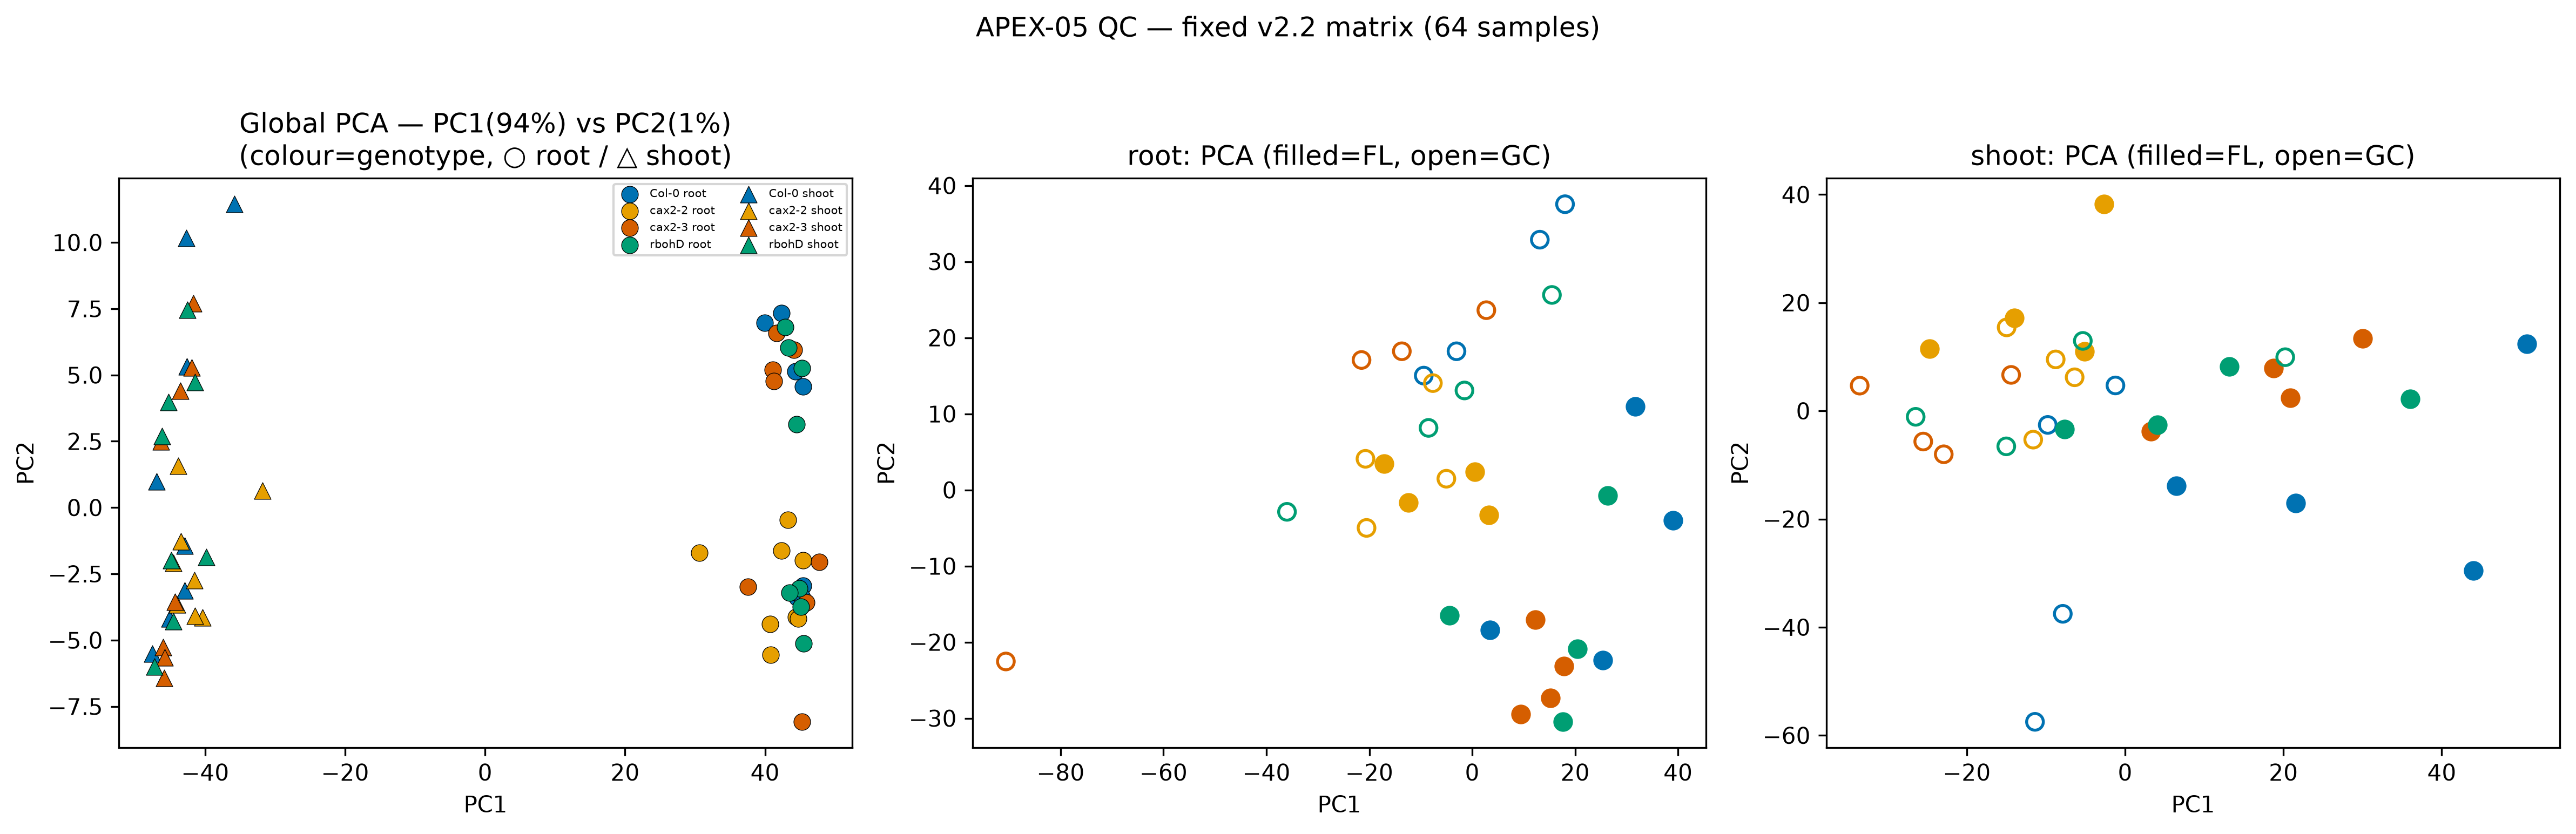
\includegraphics[width=0.85\textwidth]{figG1_qc_pca.png}
\caption{\textbf{Corrected 64-sample design and QC.} Global PCA of log2-CPM (top
2{,}000 variable genes); PC1 (94\%) separates root from shoot with no outliers, and
within-tissue FL vs GC separation is strong in Col-0/\textit{rbohD} and weak in
\textit{cax2-2}.}
\label{fig:1}
\end{figure}

\subsection{Wild-type mounts a robust flight response that CAX2 is required for}
DESeq2 (FL vs GC per genotype \(\times\) tissue; FDR \(< 0.05\), \(|\log_2\text{FC}|
> 1\)) detected a substantial wild-type response --- \textbf{Col-0 root 284 DEGs
(201 induced / 83 repressed), shoot 168 (156 / 12)} --- and a comparable
\textit{rbohD} response (root 280, shoot 33; Table~\ref{tab:deg},
Fig.~\ref{fig:2}). In sharp contrast, \textbf{\textit{cax2-2} showed almost no
transcriptional flight response: 5 root and 3 shoot DEGs} (15 / 4 even at a relaxed
1.5-fold, FDR \(< 0.1\) threshold), and its FL-vs-GC separation in
morphometric-blind PCA was \(\sim 5\times\) smaller than wild-type's (Cohen-scaled
centroid distance 7.9 vs 39.9 in root; Fig.~\ref{fig:1}). Because the sample QC was
clean, this is a genuine biological attenuation, not a data-quality artefact:
\textbf{CAX2 is required for the normal spaceflight transcriptional response.}

Wild type and \textit{rbohD} converge on a \textbf{shared 180-gene root flight
core} (of 284 and 280 DEGs respectively; Fig.~\ref{fig:s5}), whereas \textit{cax2-2}
contributes essentially nothing to it (only 2 genes shared by all three genotypes).
The shoot response is more genotype-specific (Col-0 \(\cap\) \textit{rbohD} = 4
genes). An independent machine-learning check corroborated the DESeq2 calls
(Fig.~\ref{fig:3}): a stability-selected LASSO logistic classifier separated FL from
GC at 100\% leave-one-out accuracy in every genotype, but the overlap of the LASSO
signature with the DESeq2 DEGs was strong for Col-0 and \textit{rbohD}
(hypergeometric \(p\) up to \(10^{-127}\)) and minimal for \textit{cax2-2} (5/111
root genes), mirroring its near-absent differential expression.

\begin{table}[htbp]
\centering
\caption{Spaceflight differential-expression (DESeq2, FL vs GC; FDR \(< 0.05\),
\(|\log_2\text{FC}| > 1\)) DEG counts per genotype and tissue (induced / repressed).}
\label{tab:deg}
\begin{tabular}{@{}llrrr@{}}
\toprule
\textbf{Genotype} & \textbf{Tissue} & \textbf{DEGs} & \textbf{Induced} & \textbf{Repressed} \\
\midrule
Col-0            & Root  & 284 & 201 & 83 \\
Col-0            & Shoot & 168 & 156 & 12 \\
\textit{rbohD}   & Root  & 280 & 198 & 82 \\
\textit{rbohD}   & Shoot & 33  & 2   & 31 \\
\textit{cax2-2}  & Root  & 5   & 5   & 0  \\
\textit{cax2-2}  & Shoot & 3   & 1   & 2  \\
\botrule
\end{tabular}
\par\smallskip
{\footnotesize DEG counts from \texttt{results/tables/deseq2/apex05\_deseq2\_DEG\_counts.csv}
(FDR \(< 0.05\), \(|\log_2\text{FC}| > 1\); flight-referenced). The fourth flown
genotype \textit{cax2-3} is excluded (technical artefact; see text and Fig.~\ref{fig:s1}).}
\end{table}

\begin{figure}[htbp]
\centering
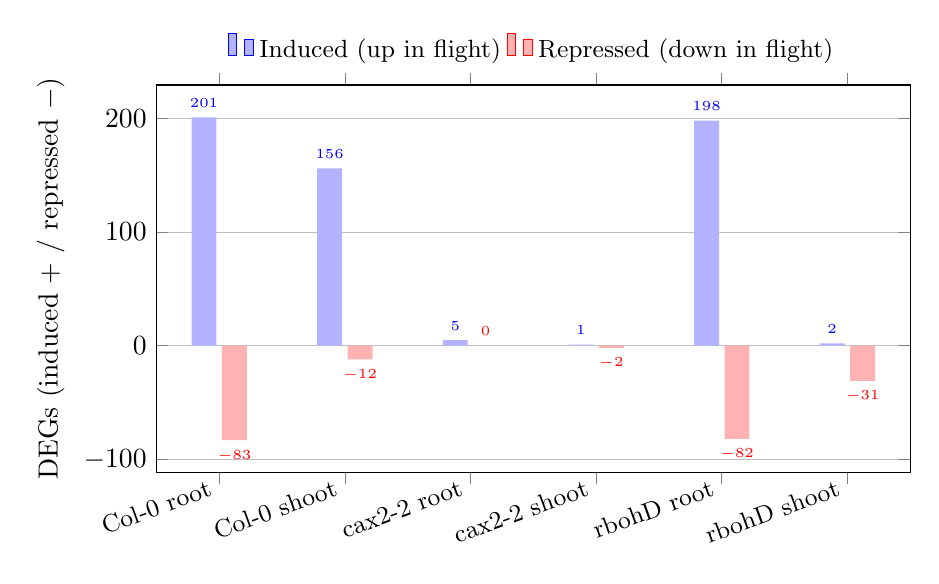
\begin{tikzpicture}
\begin{axis}[
  width=0.92\textwidth, height=6.5cm,
  ybar, bar width=9pt,
  symbolic x coords={Col-0 root,Col-0 shoot,cax2-2 root,cax2-2 shoot,rbohD root,rbohD shoot},
  xtick=data,
  x tick label style={rotate=20,anchor=east,font=\small},
  ylabel={DEGs (induced $+$ / repressed $-$)},
  ymajorgrids, enlarge x limits=0.10,
  nodes near coords, nodes near coords style={font=\tiny},
  legend style={at={(0.5,1.03)},anchor=south,legend columns=2,font=\small,draw=none},
]
\addplot+[draw=none] coordinates {(Col-0 root,201)(Col-0 shoot,156)(cax2-2 root,5)(cax2-2 shoot,1)(rbohD root,198)(rbohD shoot,2)};
\addplot+[draw=none] coordinates {(Col-0 root,-83)(Col-0 shoot,-12)(cax2-2 root,0)(cax2-2 shoot,-2)(rbohD root,-82)(rbohD shoot,-31)};
\legend{Induced (up in flight), Repressed (down in flight)}
\end{axis}
\end{tikzpicture}
\caption{\textbf{Spaceflight differential expression across genotypes.} DESeq2 DEG
counts (induced, positive; repressed, negative) per genotype \(\times\) tissue on the
corrected matrix (FDR \(< 0.05\), \(|\log_2\text{FC}| > 1\)); Col-0 and \textit{rbohD}
respond strongly, \textit{cax2-2} almost not at all. Rendered from
\texttt{results/tables/deseq2/apex05\_deseq2\_DEG\_counts.csv}.}
\label{fig:2}
\end{figure}

\begin{figure}[htbp]
\centering
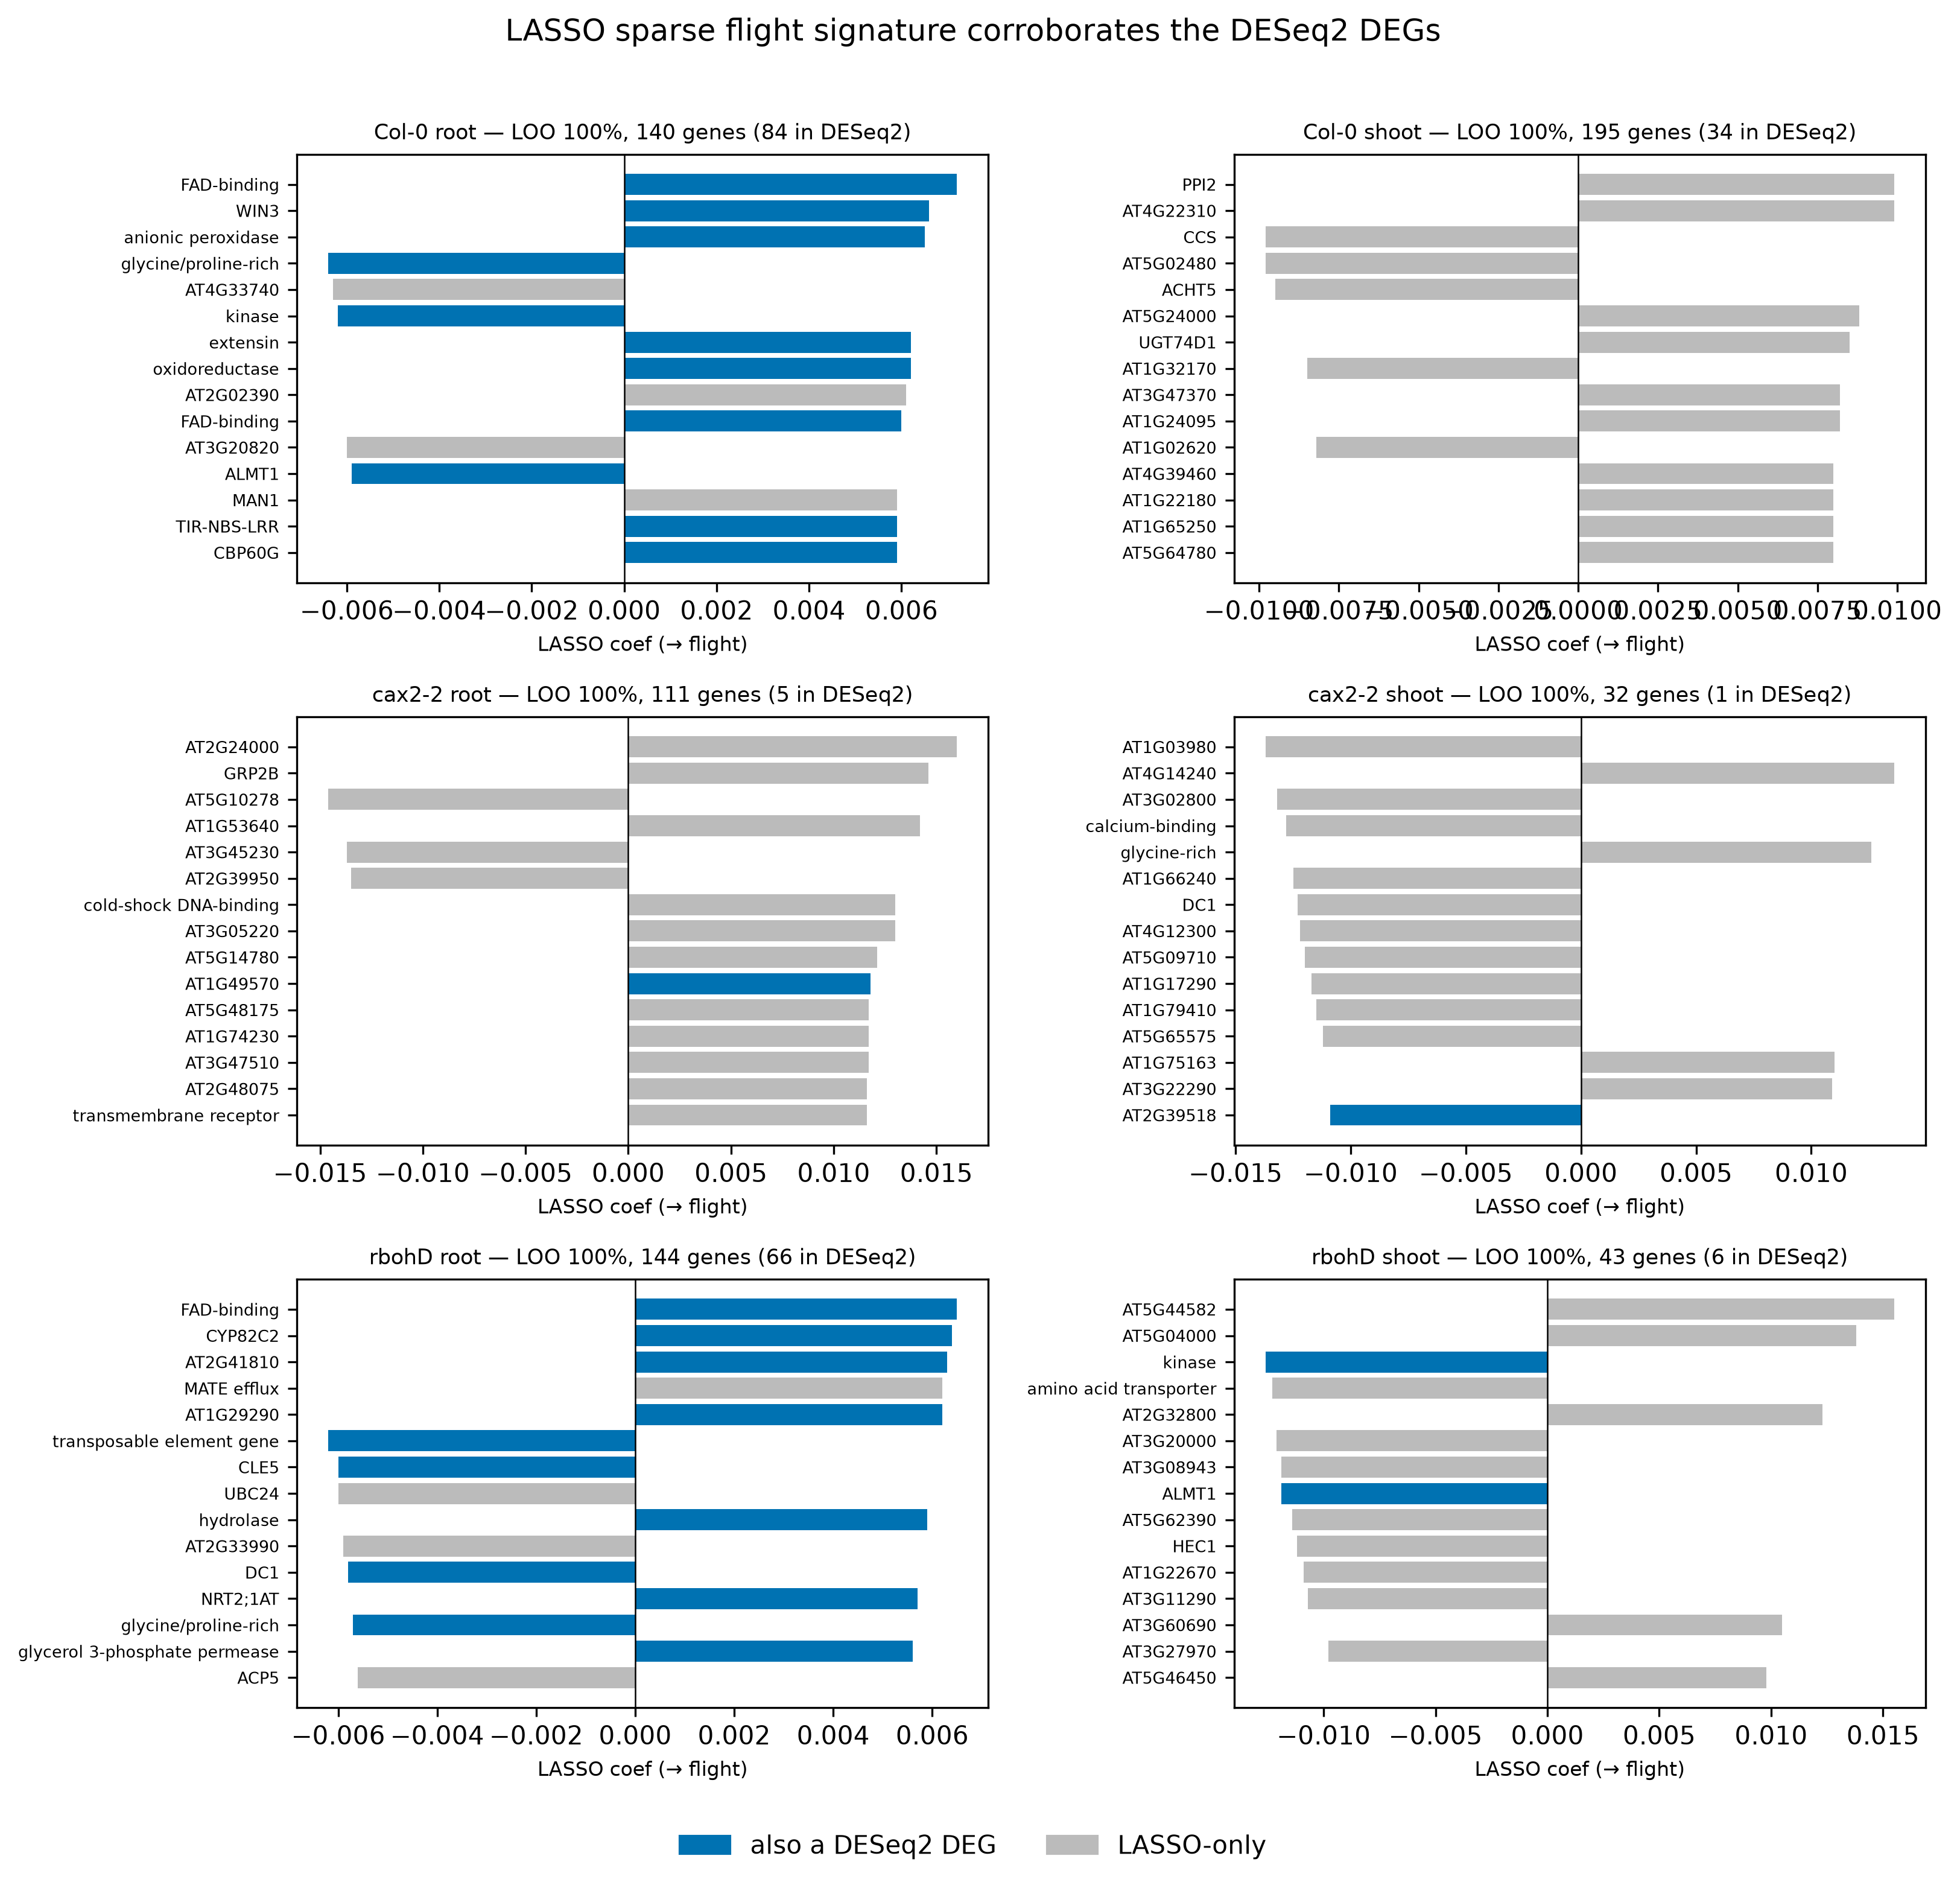
\includegraphics[width=0.85\textwidth]{figE1_lasso_flight_signature.png}
\caption{\textbf{LASSO corroborates the DESeq2 signal.} Stability-selected sparse
flight signature per genotype \(\times\) tissue; overlap with DESeq2 DEGs is strong
for Col-0/\textit{rbohD}, minimal for \textit{cax2-2}.}
\label{fig:3}
\end{figure}

\subsection{The wild-type flight response localises to the outer root and the gravity-sensing columella}
Because APEX-05 is bulk RNA-seq, we resolved the response to cell types by projecting
the DEGs onto a published \textit{A.\ thaliana} single-cell marker reference (Plant
Cell Marker DataBase, PCMDB; Fig.~\ref{fig:4}). The wild-type and \textit{rbohD}
root responses were significantly enriched for markers of the \textbf{non-hair
epidermis, cortex and columella} (Col-0 also stele; hypergeometric \(p = 8\times10^{-6}\)
to \(10^{-3}\)), with the \textit{rbohD} shoot response enriched for leaf mesophyll.
Painted onto root anatomy with ggPlantmap (Fig.~\ref{fig:5}), the response occupies
the outer root layers in Col-0 and \textit{rbohD} and is \textbf{blank in
\textit{cax2-2}}. The enrichment of the \textbf{columella --- the root's
gravity-sensing statolith tissue} --- is notable for a microgravity experiment.

\begin{figure}[htbp]
\centering
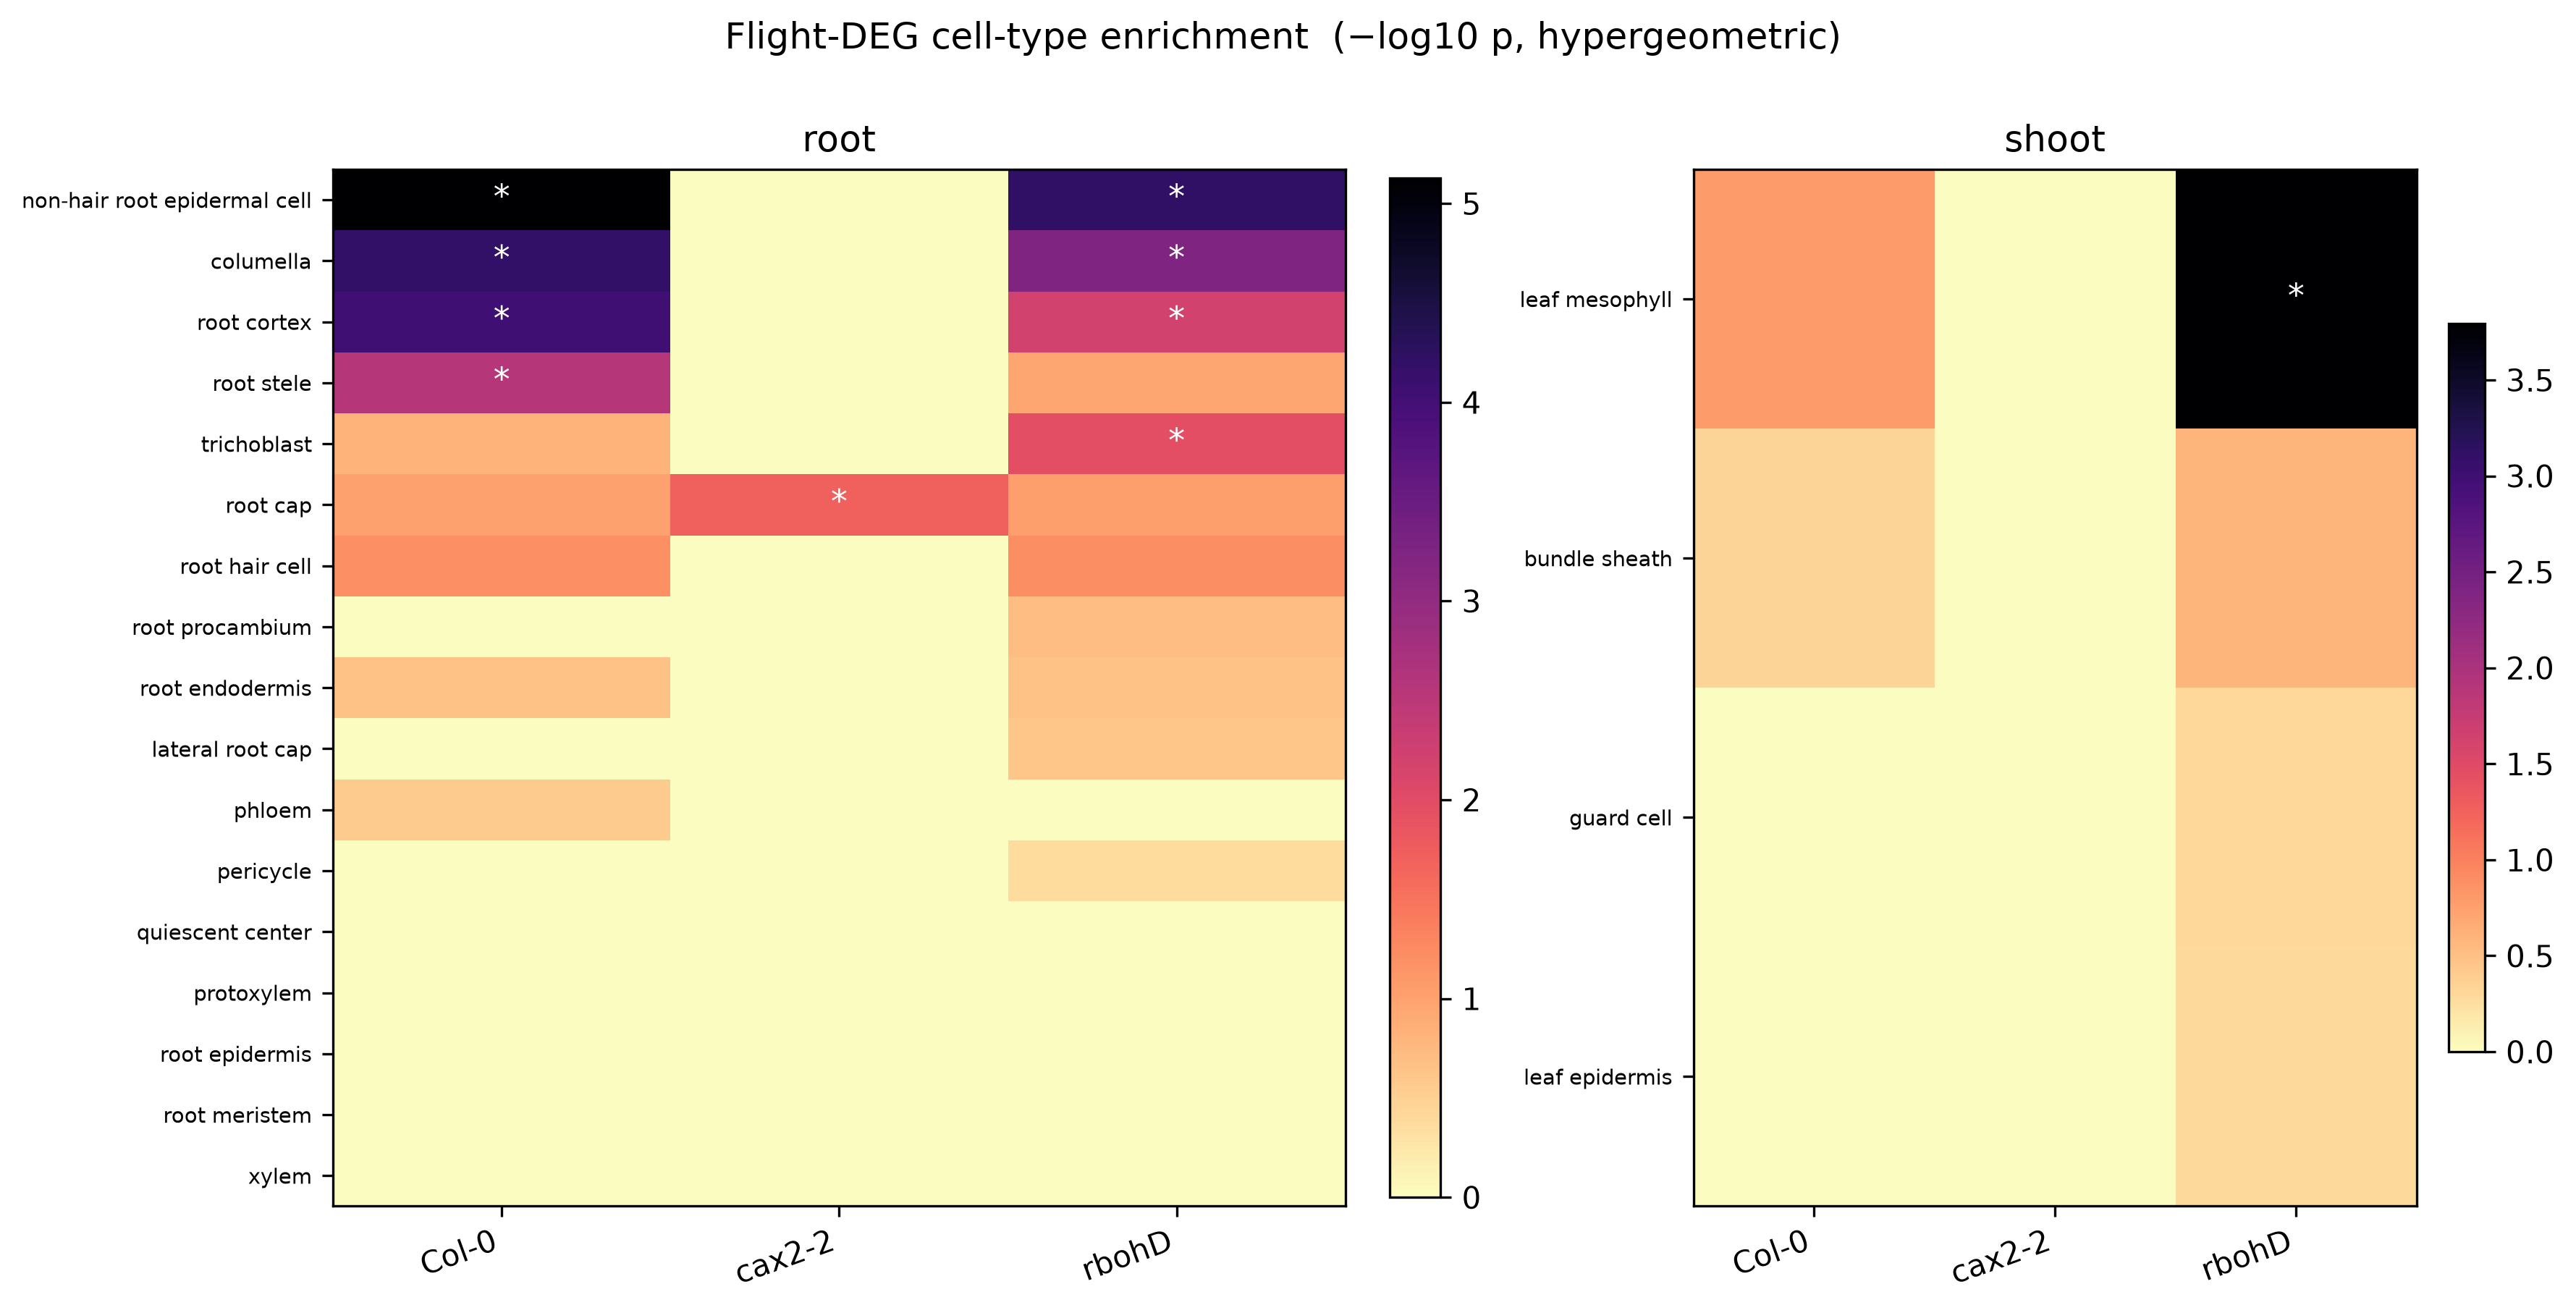
\includegraphics[width=0.48\textwidth]{figH1_celltype_deg_enrichment.png}\hfill
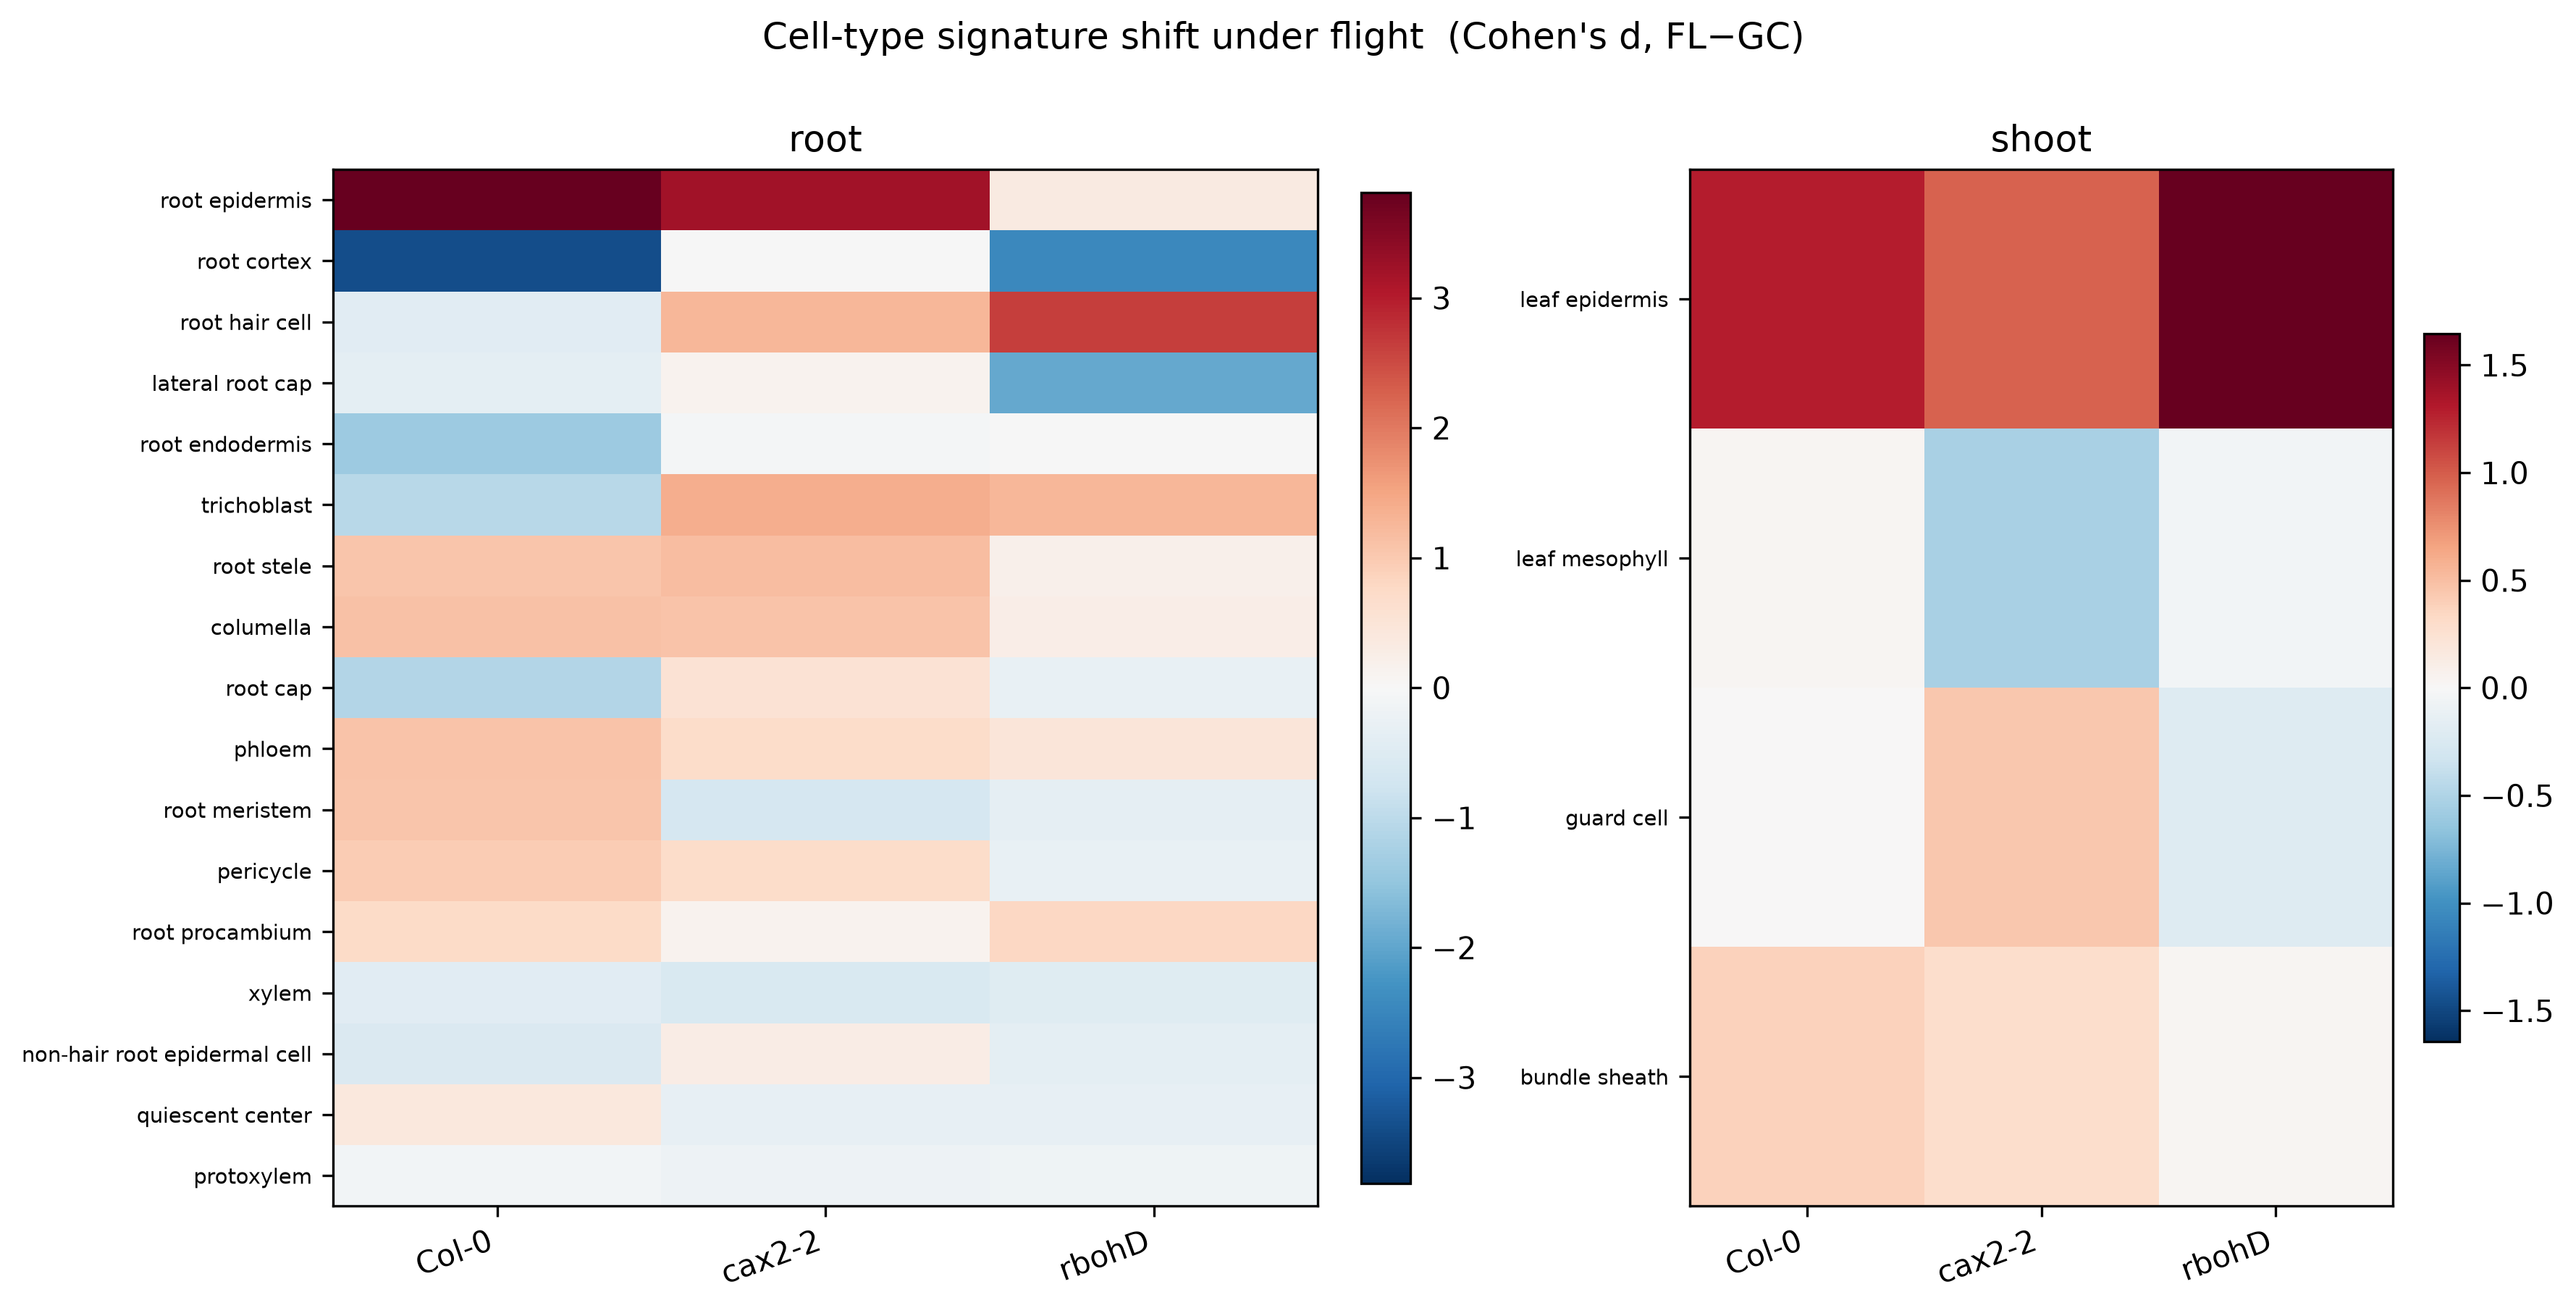
\includegraphics[width=0.48\textwidth]{figH2_celltype_signature_shift.png}
\caption{\textbf{Cell-type enrichment of the flight response (PCMDB projection).}
Hypergeometric enrichment of flight DEGs in cell-type marker sets; Col-0/\textit{rbohD}
root \(\to\) epidermis, columella, cortex; \textit{rbohD} shoot \(\to\) mesophyll;
\textit{cax2-2} flat. Right: cell-type signature shift.}
\label{fig:4}
\end{figure}

\begin{figure}[htbp]
\centering
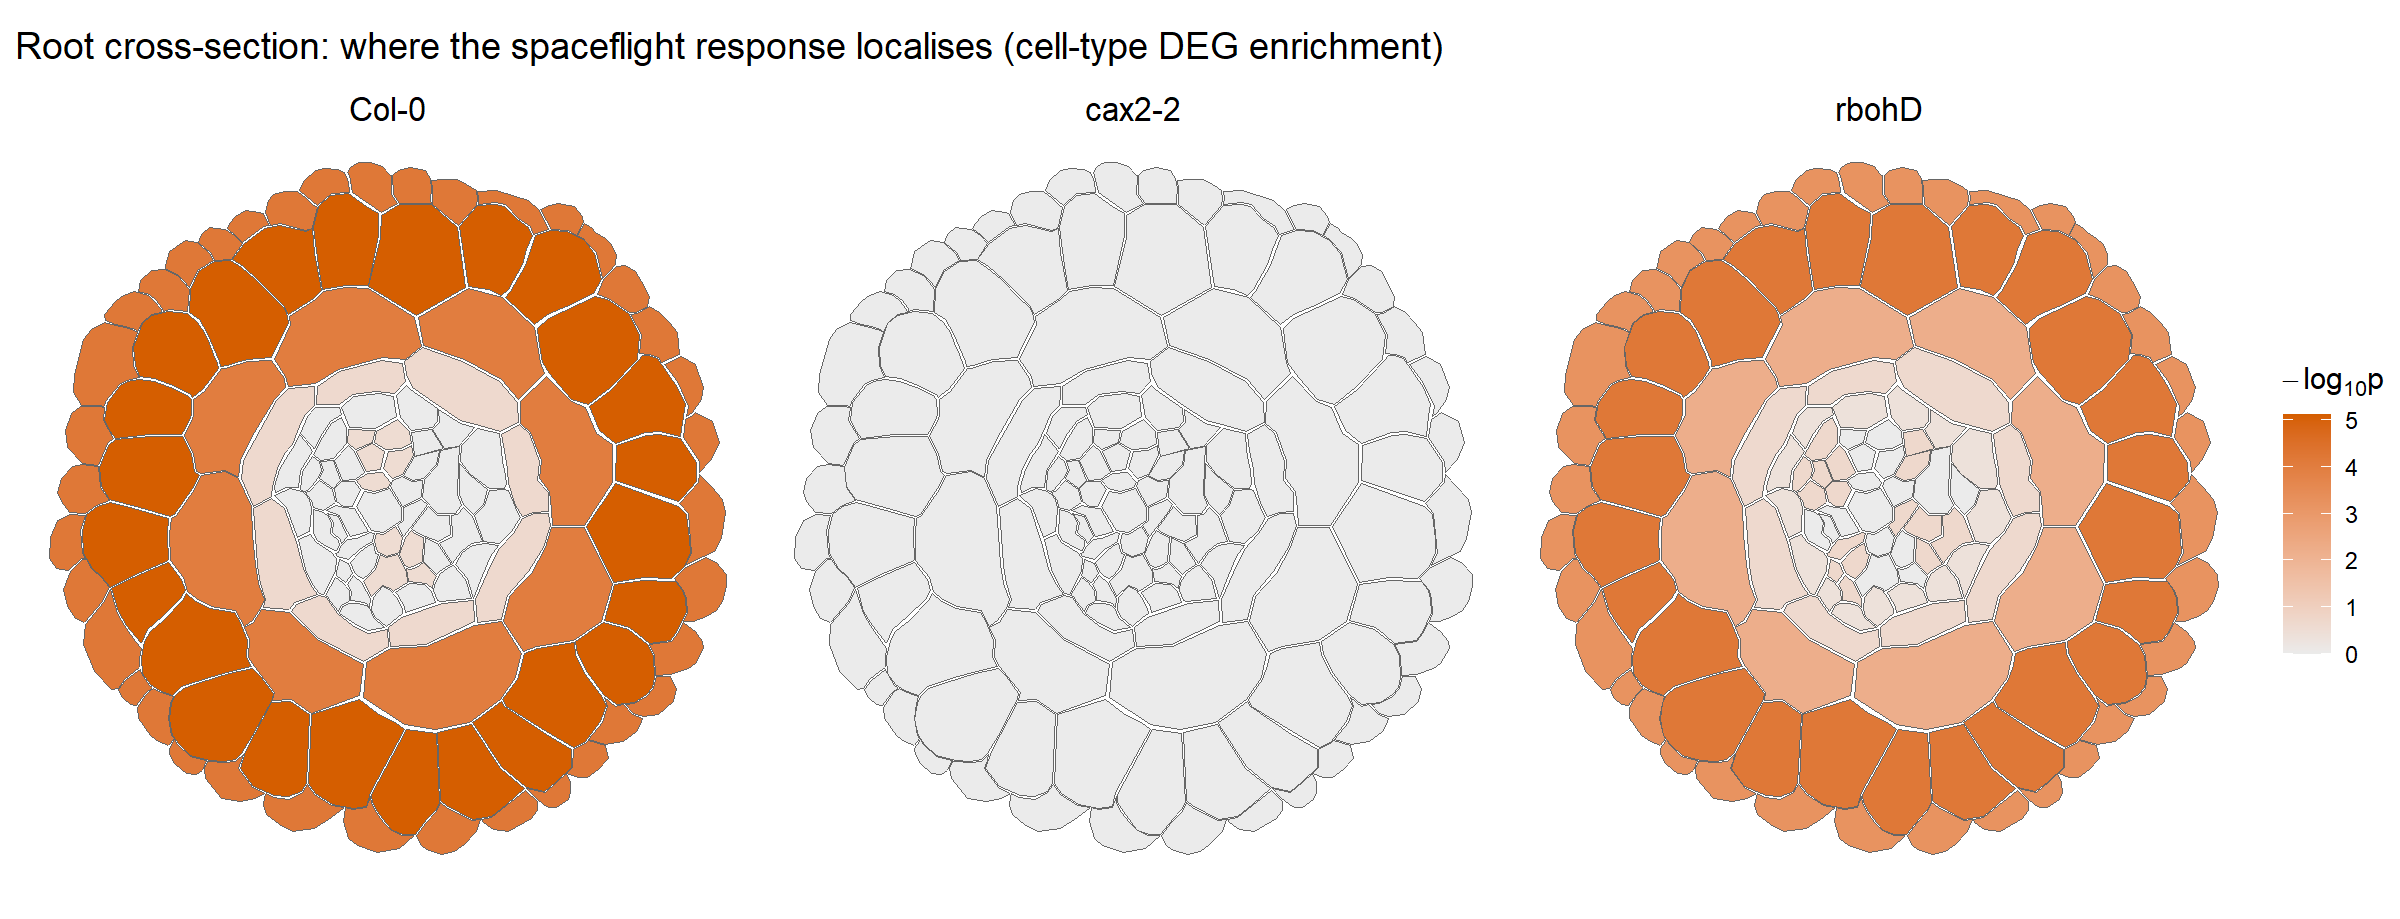
\includegraphics[width=0.48\textwidth]{figM1_root_anatomy_flight.png}\hfill
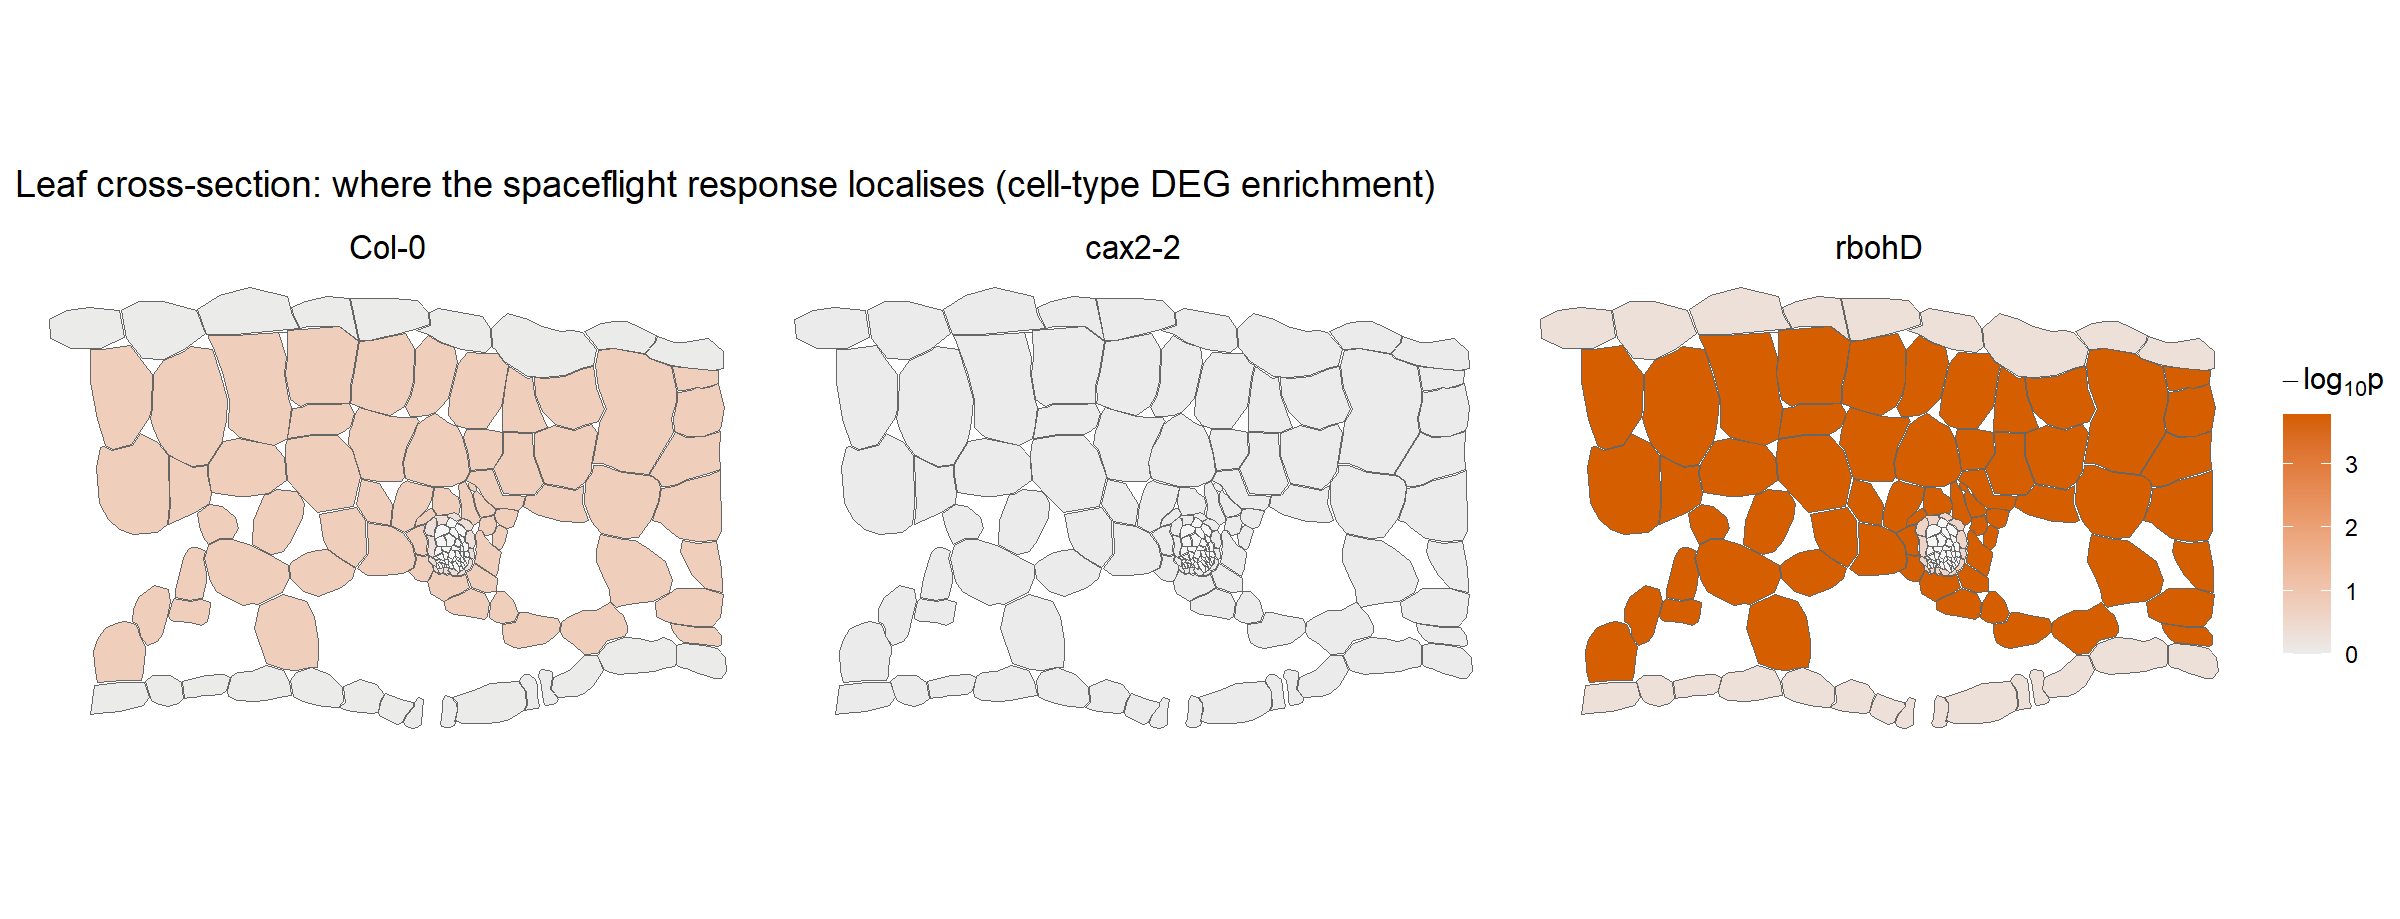
\includegraphics[width=0.48\textwidth]{figM2_leaf_anatomy_flight.png}
\caption{\textbf{Anatomical localisation (ggPlantmap).} Root (left) and leaf (right)
cross-section painted by cell-type flight enrichment: outer-root (epidermis+cortex)
in Col-0/\textit{rbohD}, blank in \textit{cax2-2}.}
\label{fig:5}
\end{figure}

\subsection{Spaceflight remodels root architecture in all genotypes, uncoupling expression from growth}
From the same wells, day-4 primary-root morphometrics showed that \textbf{spaceflight
significantly shortened roots and reduced root surface and volume in every genotype}
(length/vector-length/surface/volume Cohen's \textit{d} \(\approx -0.3\) to \(-1.5\),
all \(p < 0.05\); \textit{rbohD} strongest and also thinner, diameter \textit{d} =
\(-0.69\); Fig.~\ref{fig:6}). Integrating the two modalities per well revealed a key
dissociation: although \textit{cax2-2} is the weakest responder in both assays, its
transcriptome is \textbf{disproportionately attenuated relative to its retained
root-shortening} (root DEGs 5 vs Col-0 284, but morphometric mean \(|d|\) 0.67 vs
0.86). Thus in \textit{cax2-2} the morphological flight response proceeds largely
without the transcriptional one --- \textbf{CAX2 is required chiefly for the
transcriptional arm of the response.}

The position-paired design allowed this dissociation to be tested at finer
resolution (Fig.~\ref{fig:6}c): across the 12 primary-genotype root wells, the
per-well transcriptomic flight magnitude (mean \(|\Delta\log_2\text{CPM}|\) over the
flight-DEG panel) and the per-well root-shortening (\(|\Delta\) root length\(|\))
were \textbf{not correlated} (Spearman \(\rho = -0.30\), \(p = 0.34\)), and no
individual flight-DEG's per-well expression change tracked root-shortening after FDR
correction (0 / 385 genes at BH-FDR \(< 0.1\)). The transcriptomic axis cleanly
separated \textit{cax2-2} (low) from Col-0/\textit{rbohD} (high), whereas
root-shortening overlapped across all three --- confirming, at well and gene
resolution, that the spaceflight root-growth response is largely \textbf{uncoupled}
from the measured transcriptional response.

\begin{figure}[htbp]
\centering
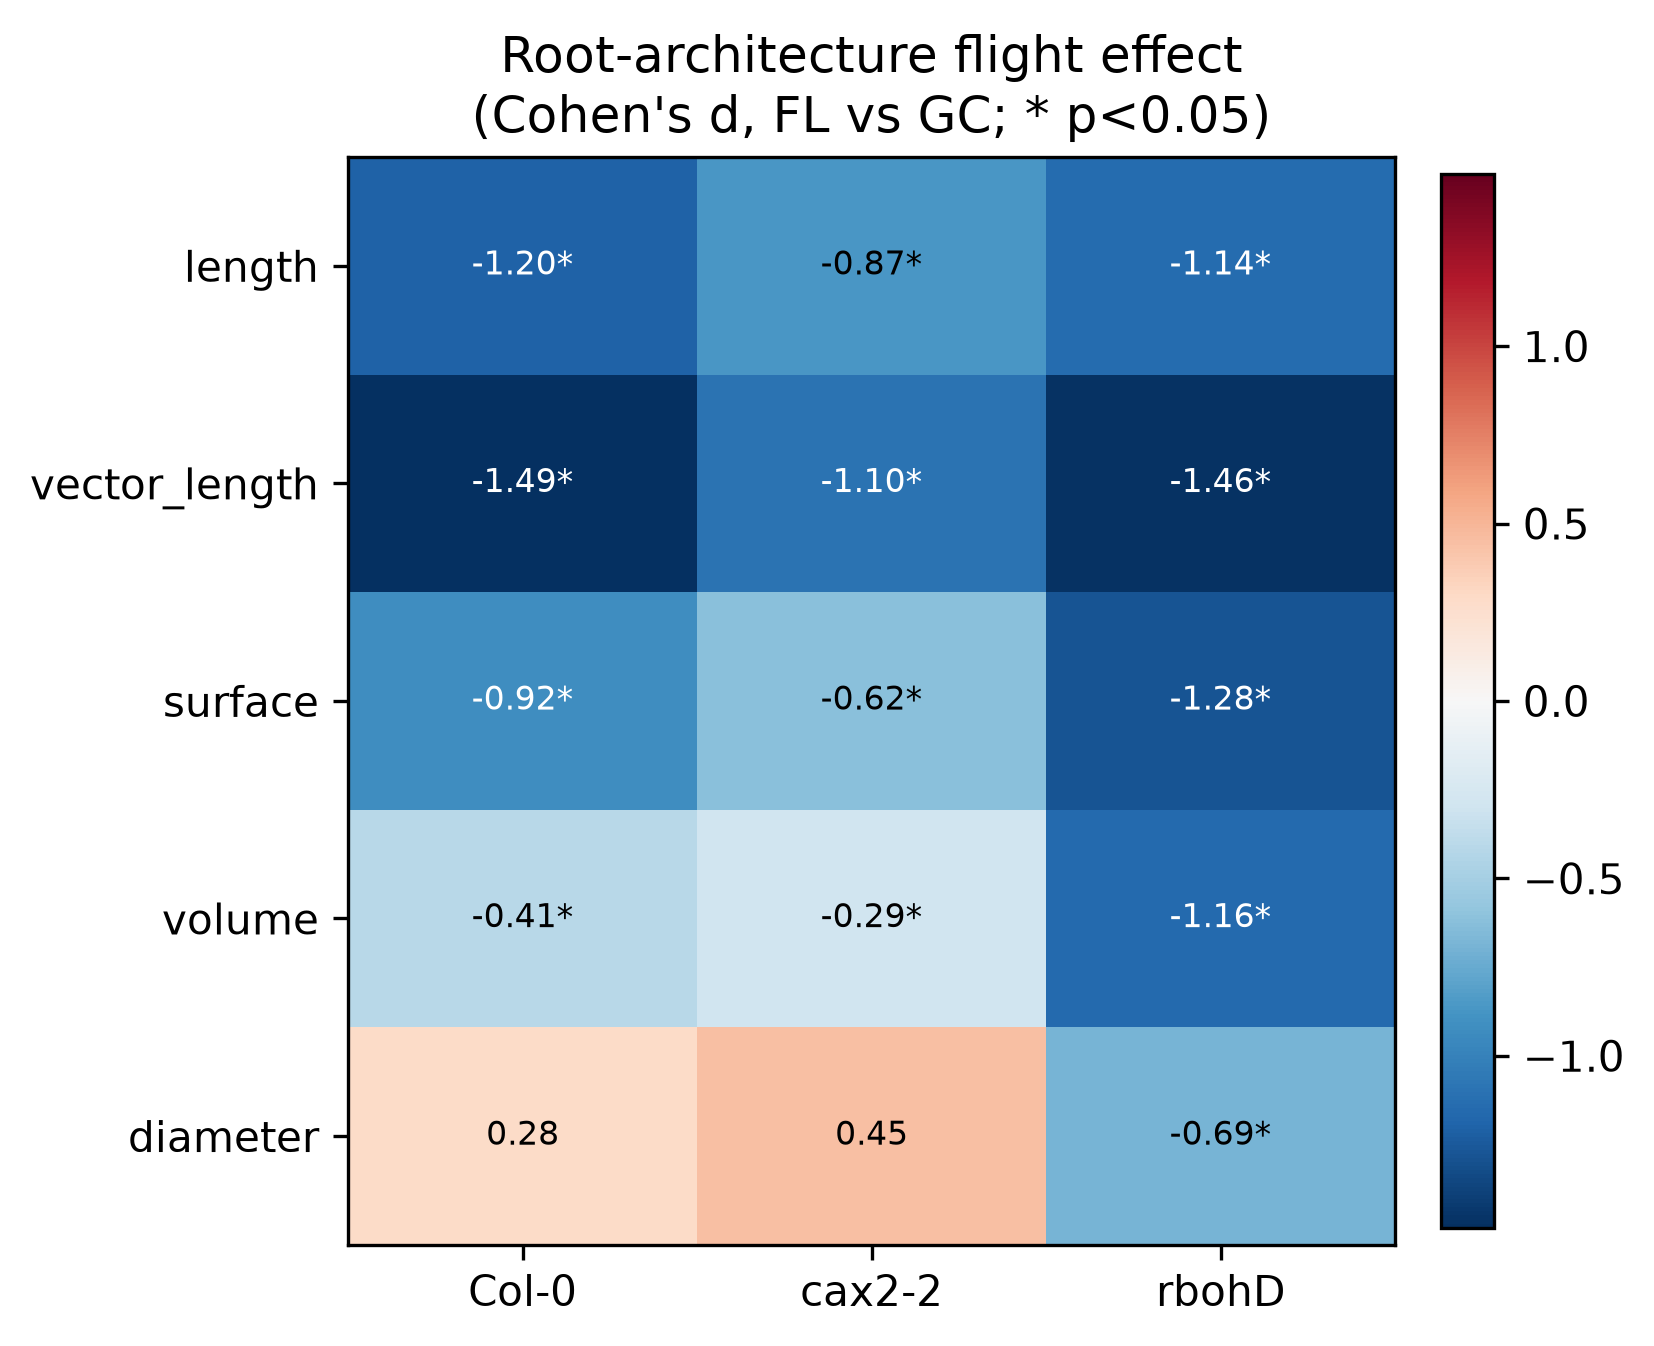
\includegraphics[width=0.32\textwidth]{figI1_morphometric_flight_effects.png}\hfill
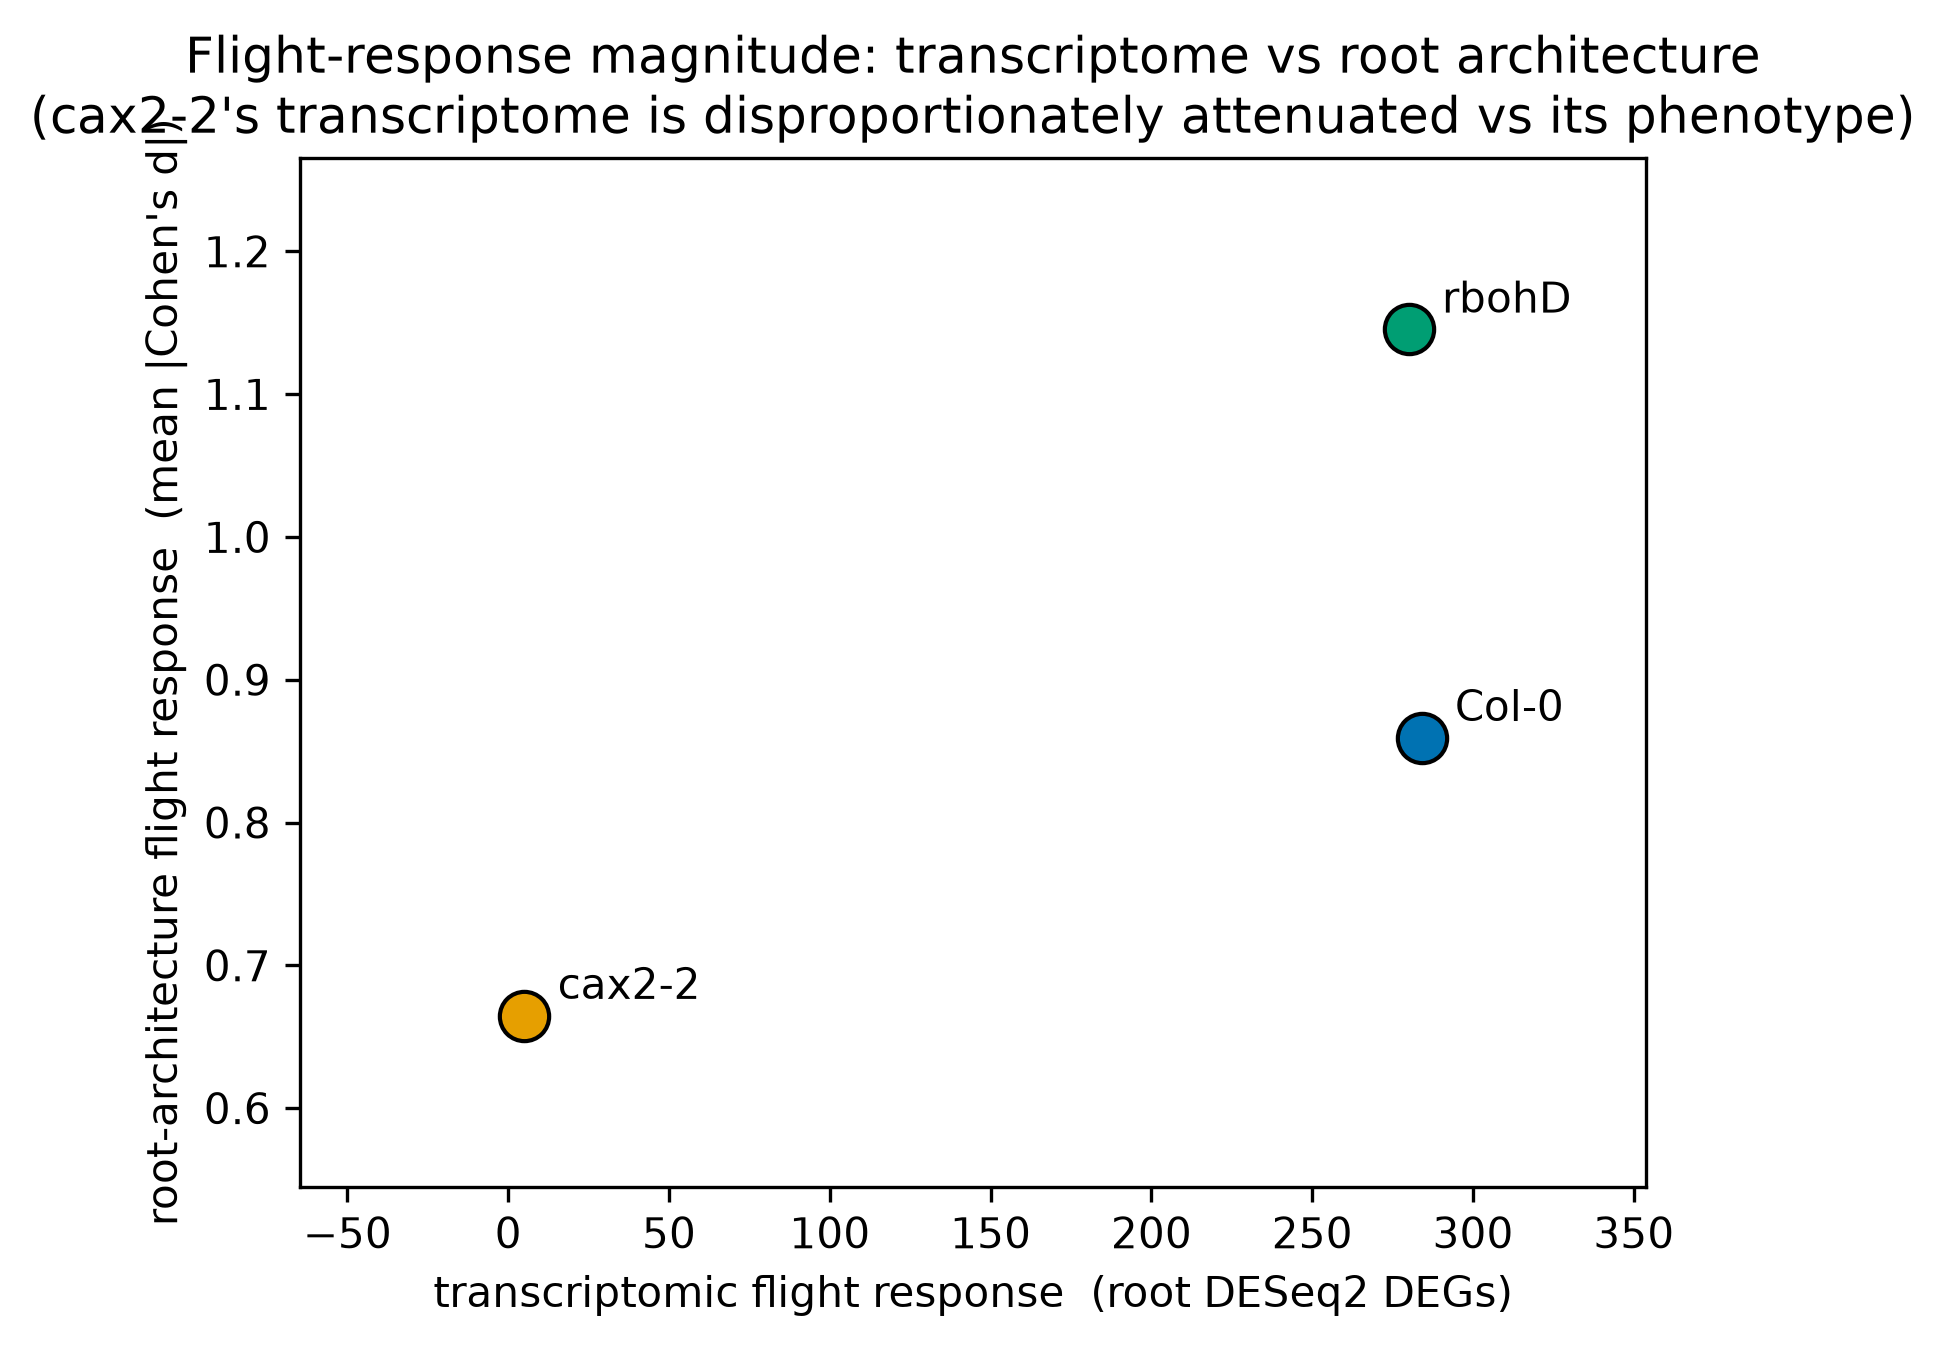
\includegraphics[width=0.32\textwidth]{figI2_transcriptome_vs_phenotype.png}\hfill
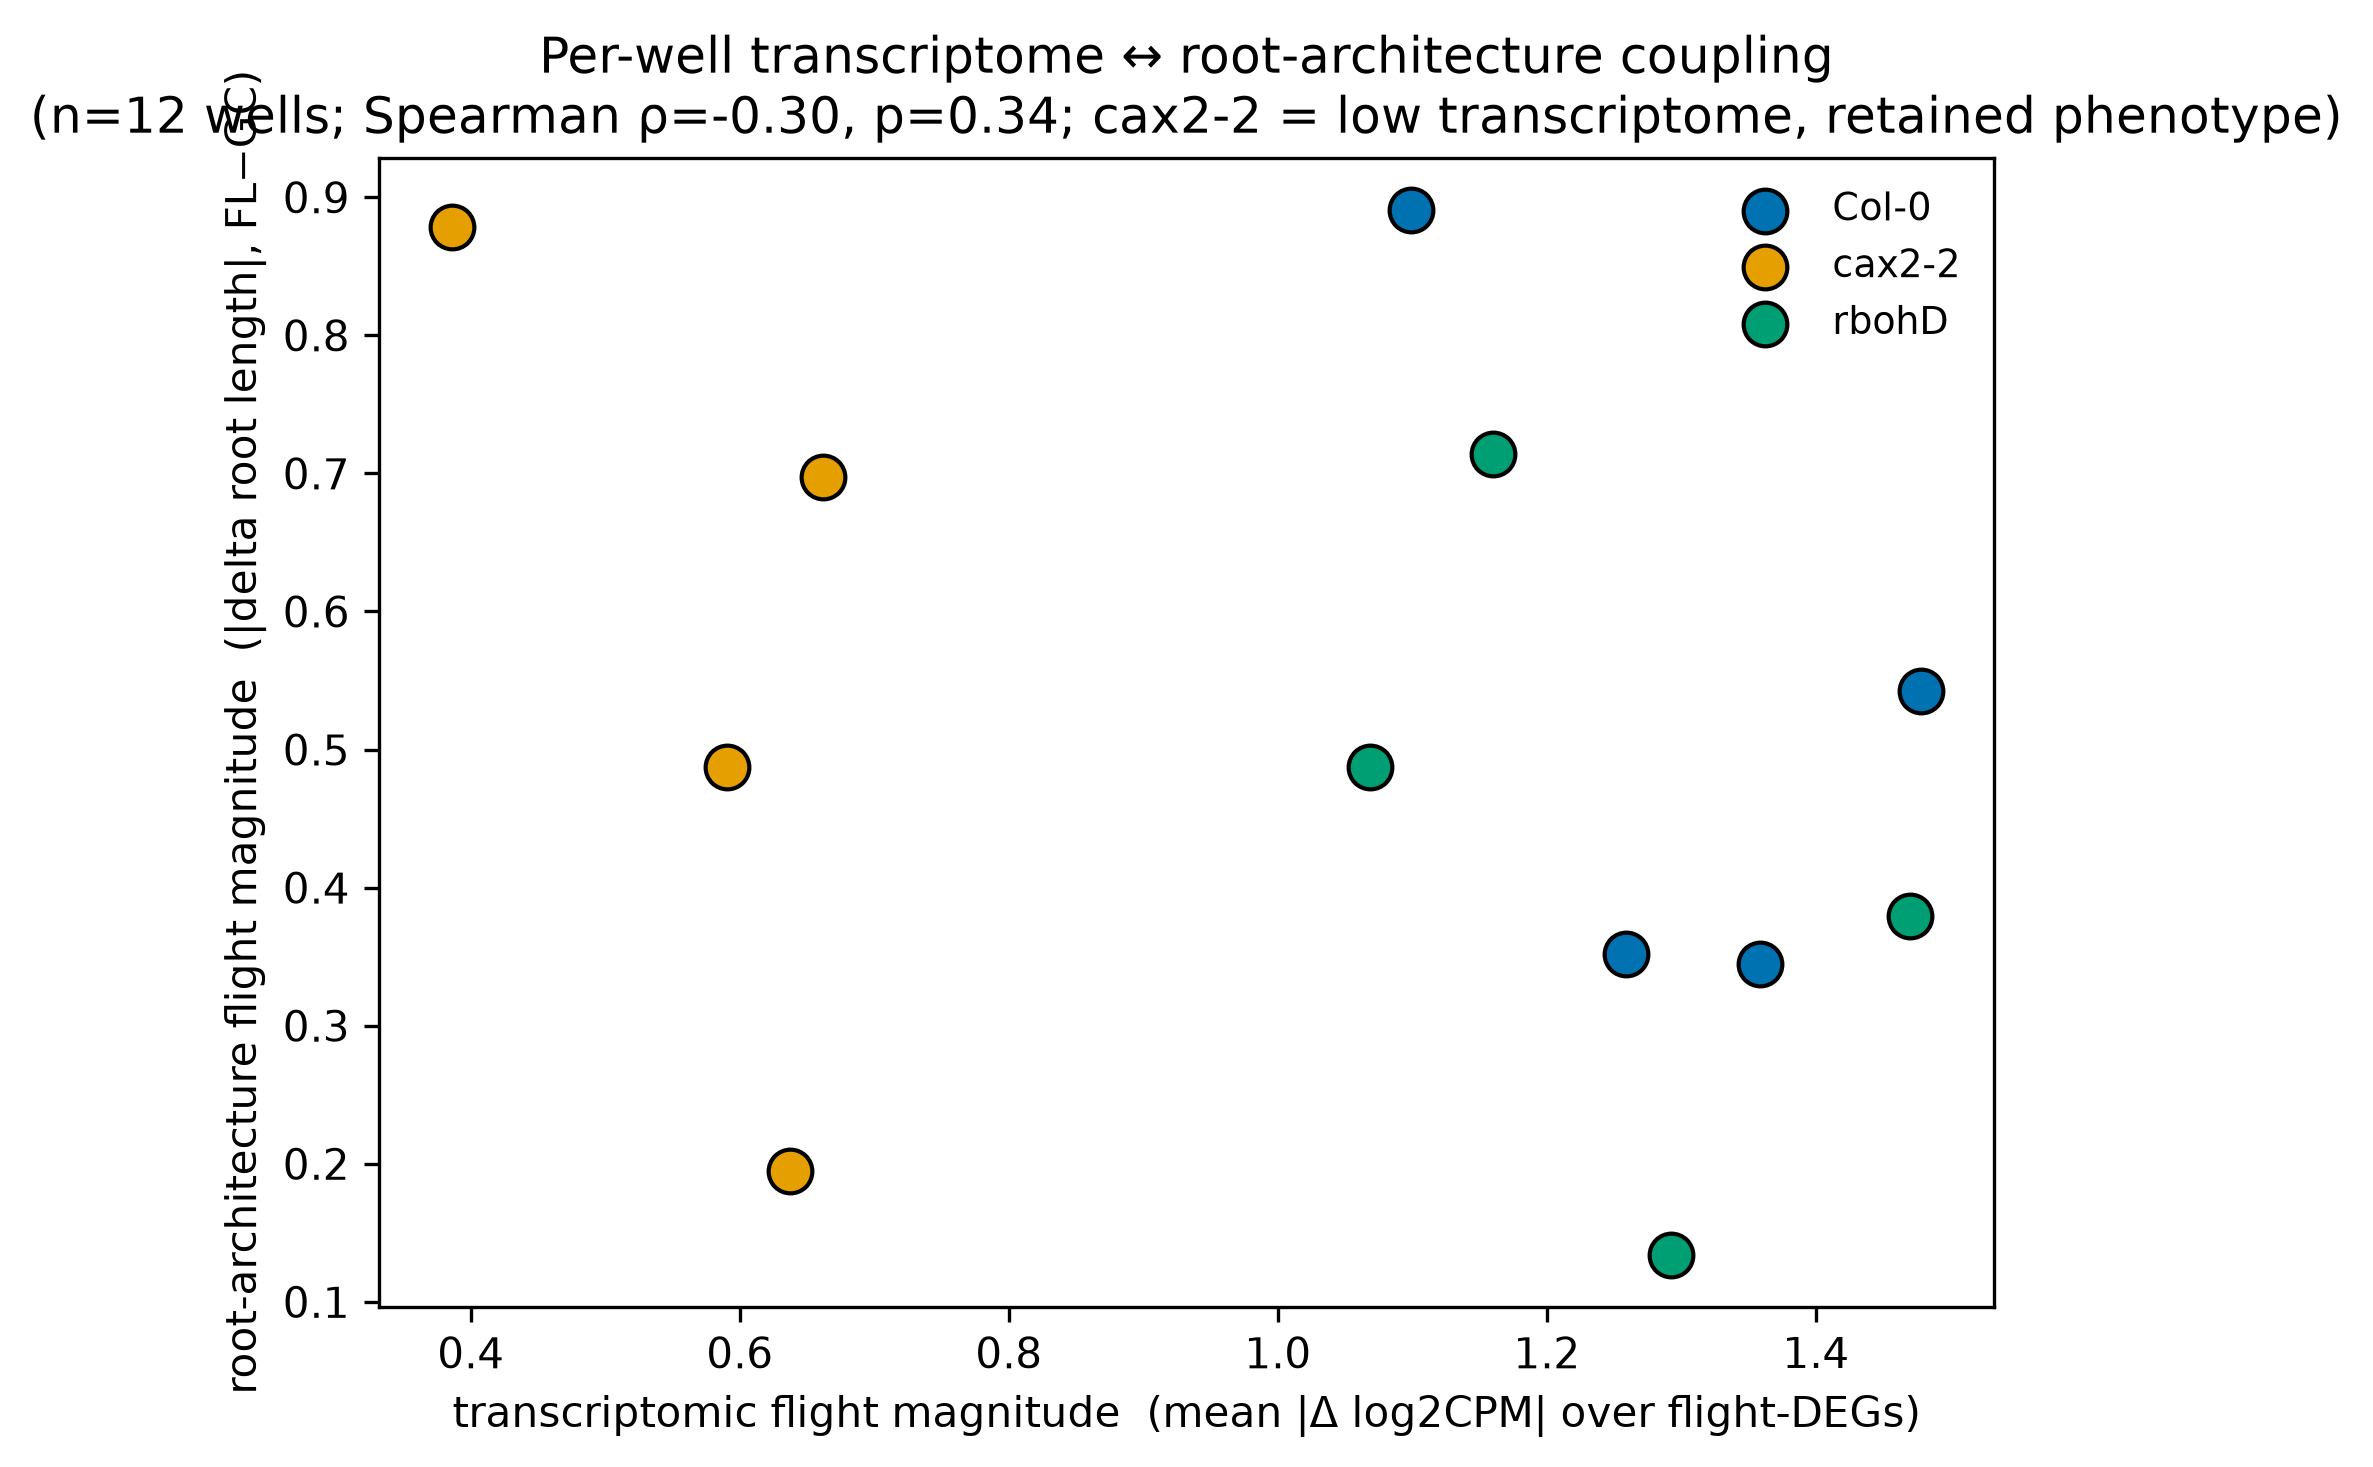
\includegraphics[width=0.32\textwidth]{figI3_welllevel_coupling.png}
\caption{\textbf{Root-architecture flight response and multi-omics integration.}
(a) Morphometric flight effects (Cohen's \textit{d}, FL vs GC); roots shorten in all
genotypes. (b) Transcriptome vs phenotype magnitude (genotype level) ---
\textit{cax2-2}'s transcriptome is disproportionately attenuated relative to its
retained root-shortening. (c) Per-well coupling (\(n = 12\) root wells): per-well
transcriptomic flight magnitude vs \(|\Delta\) root length\(|\) are uncorrelated
(Spearman \(\rho = -0.30\), \(p = 0.34\)).}
\label{fig:6}
\end{figure}

\subsection{The flight response resembles hypoxia, oxidative and defence stress}
A stress-resemblance analysis (GO ``response to'' over-representation, per organ;
Fig.~\ref{fig:7}) found the wild-type and \textit{rbohD} flight DEGs most resembled
\textbf{hypoxia, oxidative/ROS and defence (salicylate/jasmonate/wounding)} stress
programmes --- all documented features of plant spaceflight --- while \textit{cax2-2}
matched none. The resemblance was \textbf{organ-specific}: the \textbf{root} response
decoded predominantly to \textbf{hypoxia and oxidative/ROS}, whereas the
\textbf{shoot} response decoded to \textbf{defence/immune} programmes (biotic,
salicylate in Col-0; jasmonate and wounding in \textit{rbohD}). A cell-type-resolved
decoding (Fig.~\ref{fig:s3}) localised the defence/hormone signature chiefly to the
\textbf{leaf mesophyll}. Systems-level KEGG analysis (Fig.~\ref{fig:8}) showed Col-0
and \textit{rbohD} root responses converging on \textbf{glutathione metabolism and
phenylpropanoid biosynthesis}; the phenylpropanoid/lignin pathway was broadly
flight-induced in the Col-0 shoot. \textit{rbohD}'s prominent glutathione-transferase
and oxidoreductase signature is consistent with its role in redox homeostasis.

\begin{figure}[htbp]
\centering
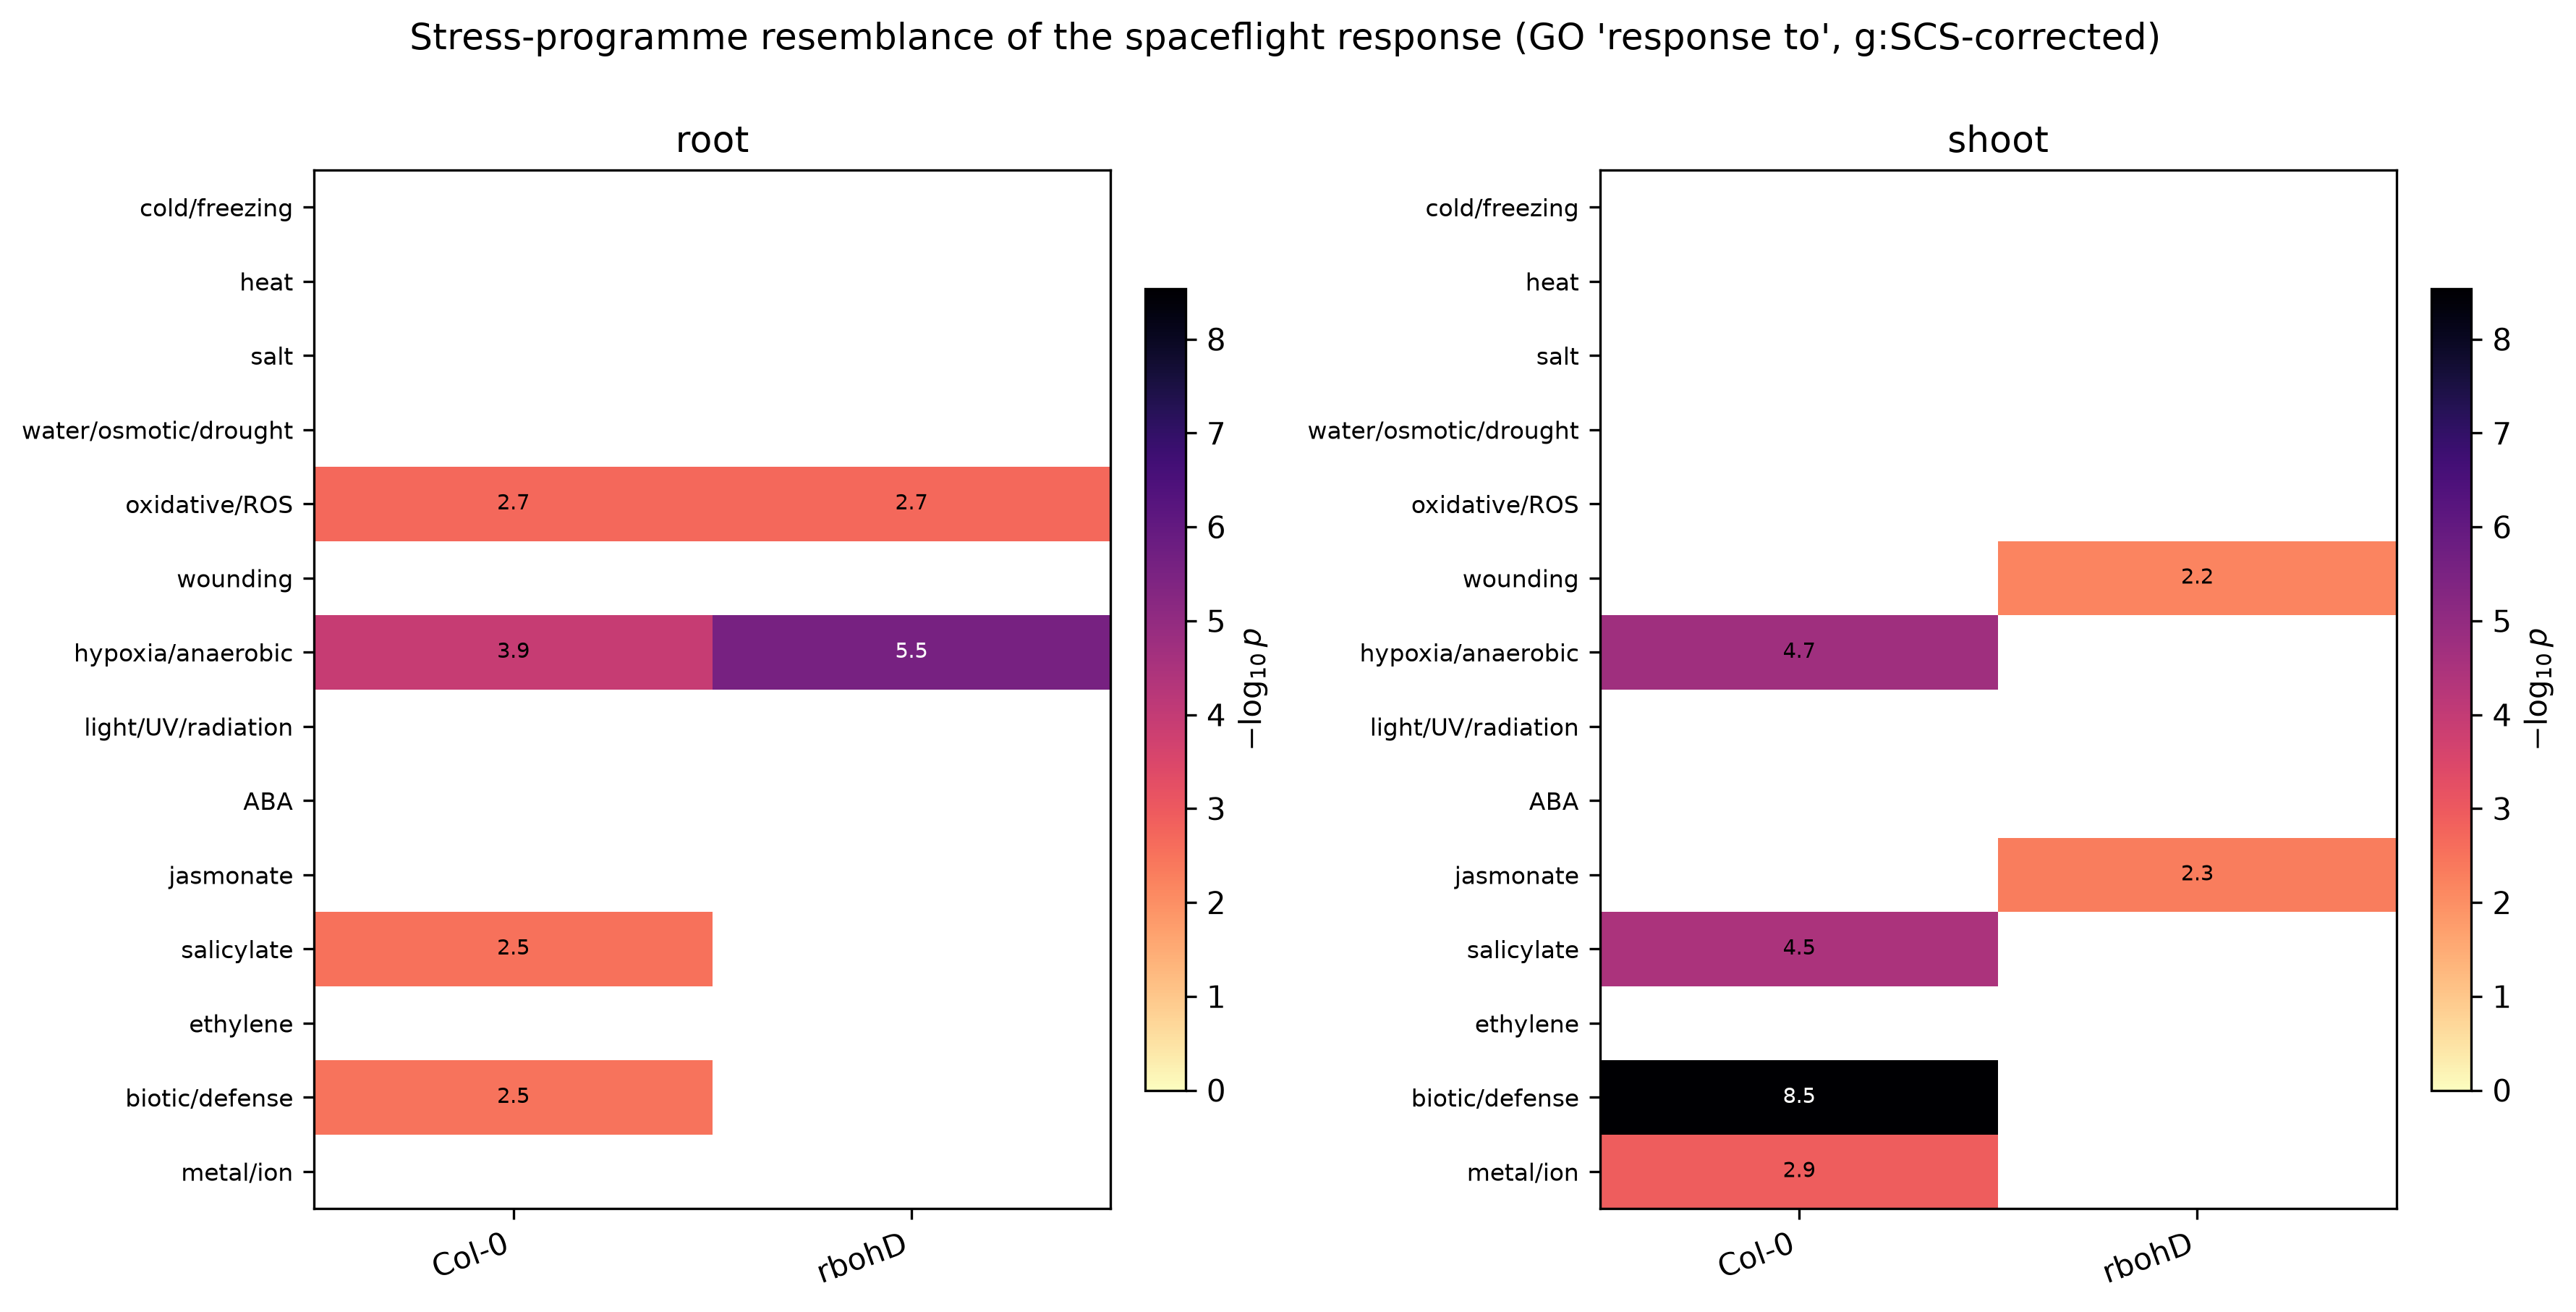
\includegraphics[width=0.85\textwidth]{figL1_stress_resemblance.png}
\caption{\textbf{Stress-programme resemblance (per organ).} GO ``response to''
over-representation grouped into stress axes, computed separately for root and shoot:
the root flight response resembles hypoxia and oxidative/ROS, the shoot response
resembles defence/salicylate/jasmonate/wounding; \textit{cax2-2} matches none.}
\label{fig:7}
\end{figure}

\begin{figure}[htbp]
\centering
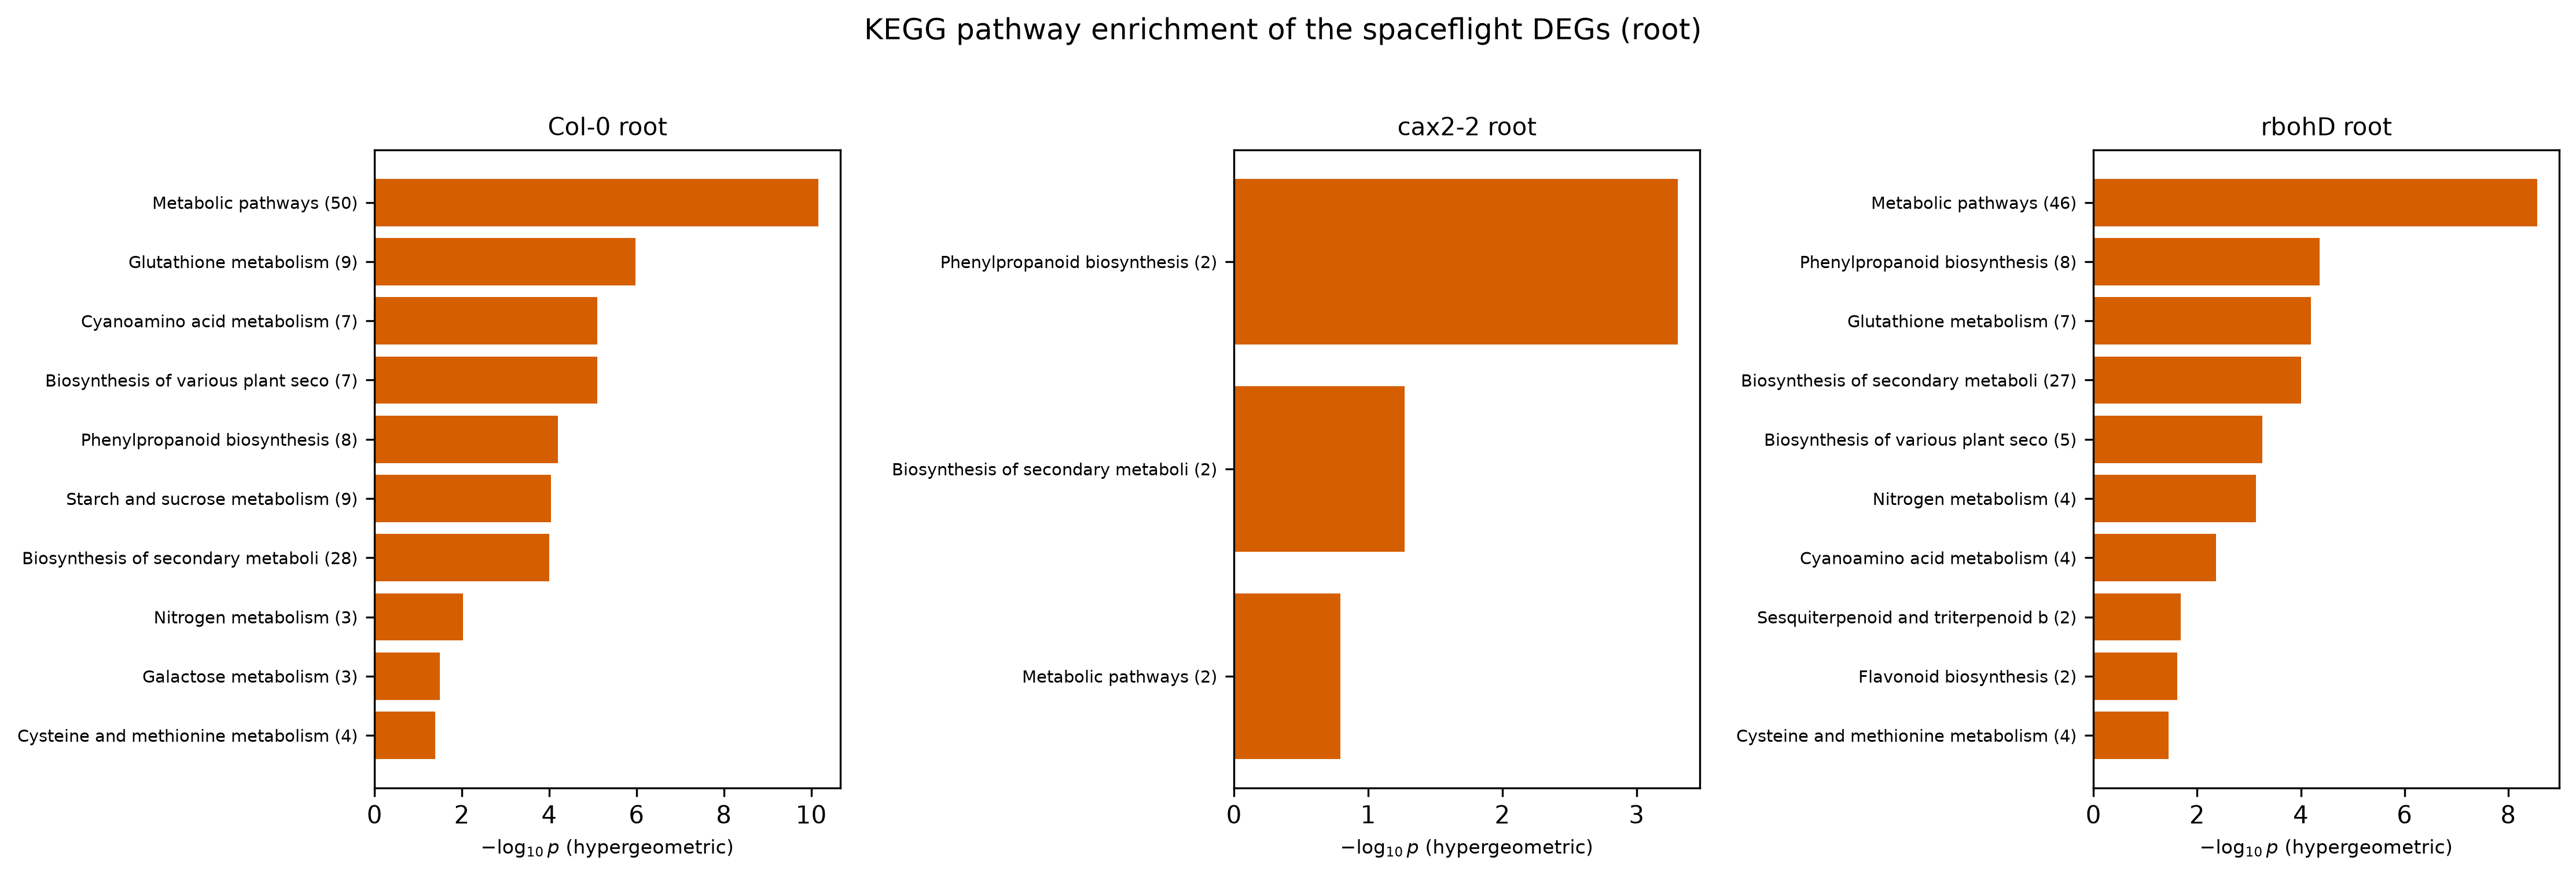
\includegraphics[width=0.7\textwidth]{figK1_kegg_pathway_enrichment.png}\\[1ex]

\includegraphics[width=0.32\textwidth]{figJ_ath00940_col0_shoot.png}\hfill
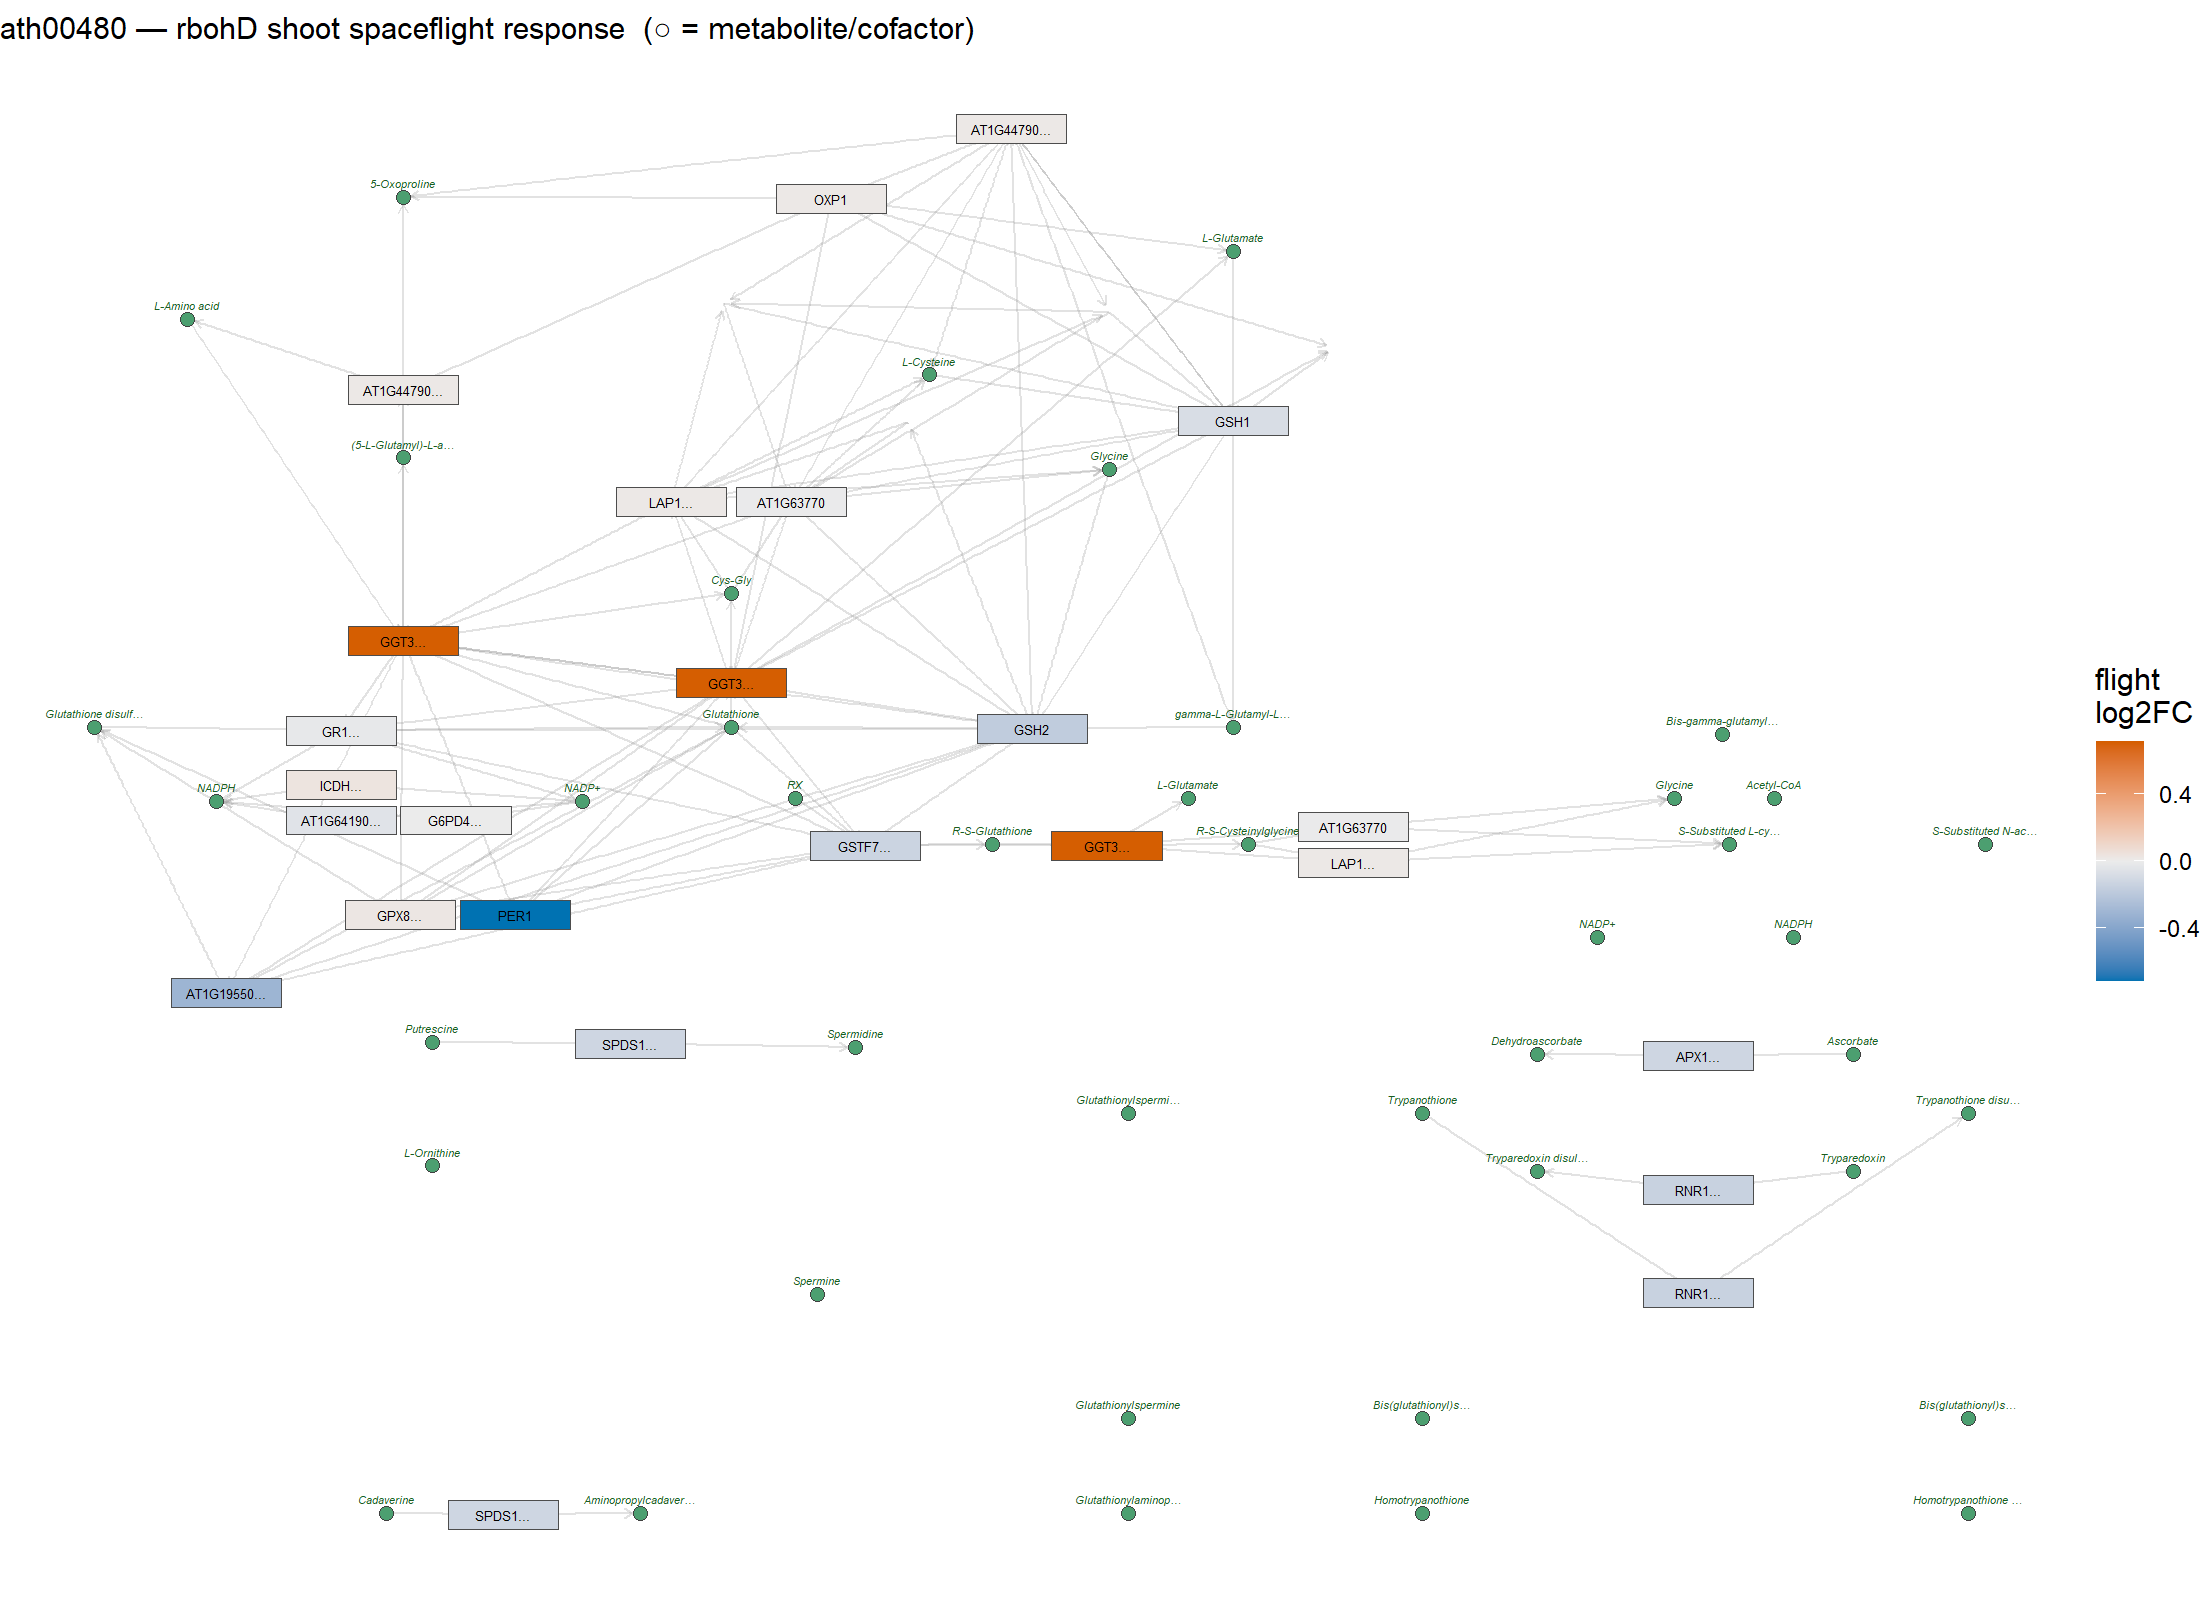
\includegraphics[width=0.32\textwidth]{figJ_ath00480_rbohd_shoot.png}\hfill
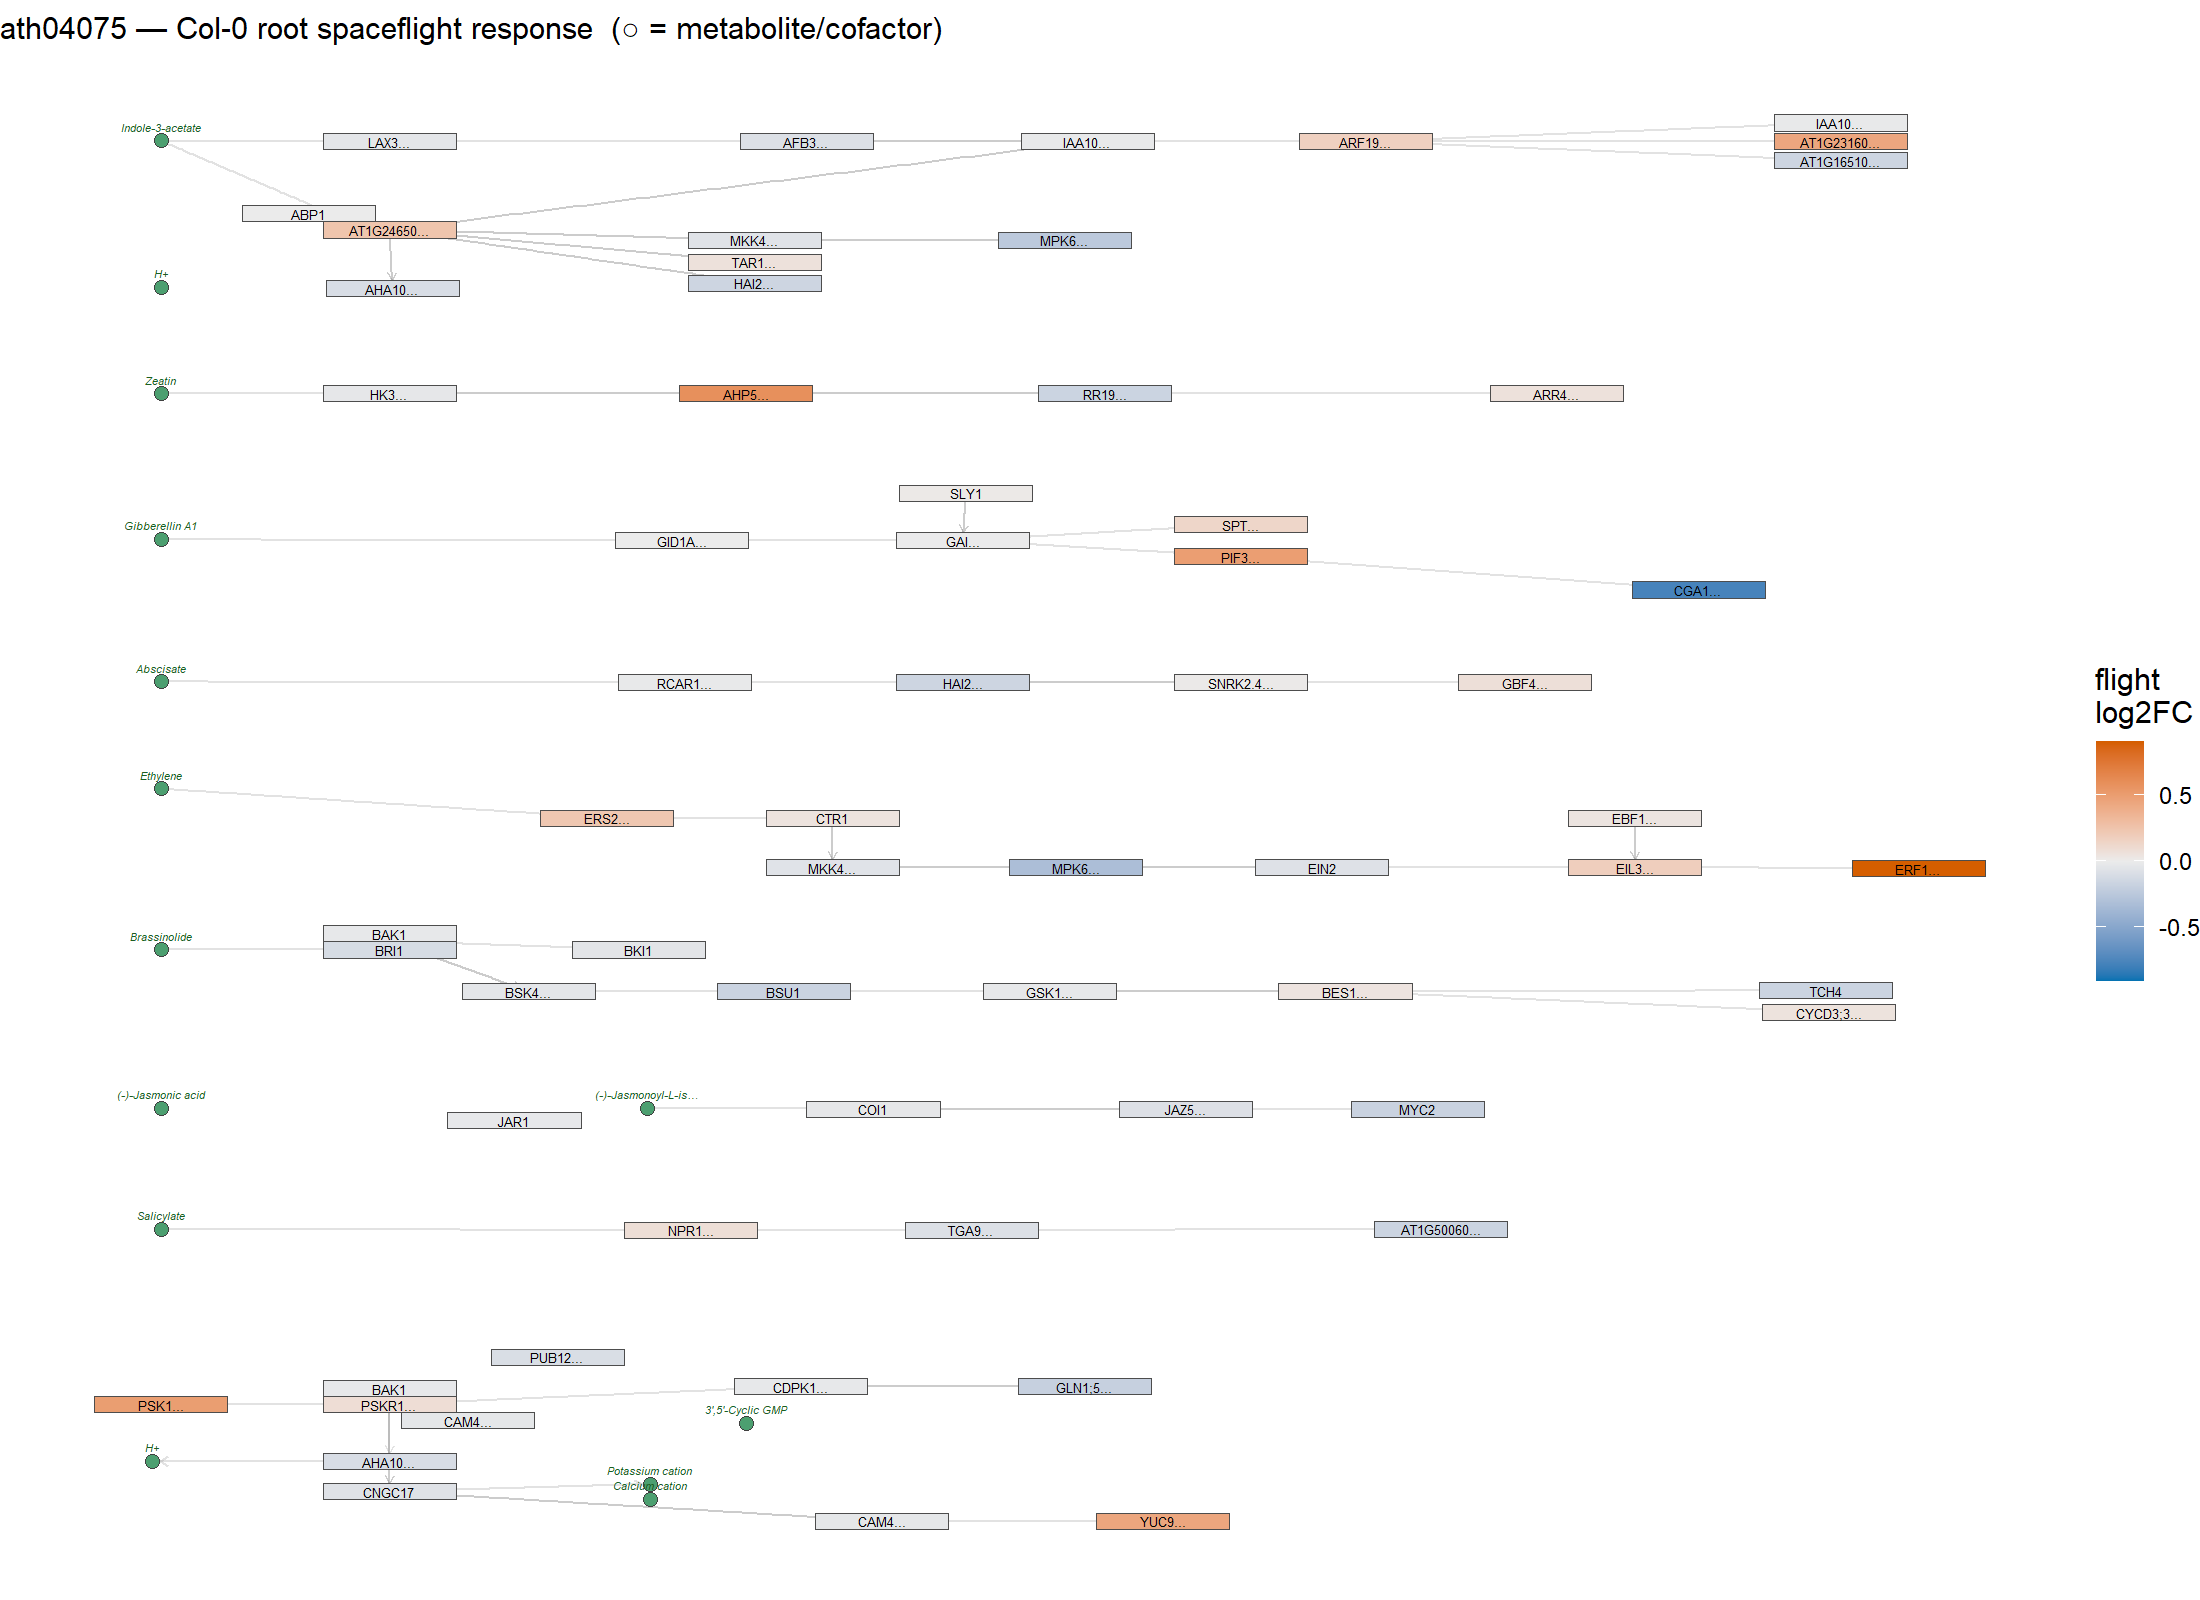
\includegraphics[width=0.32\textwidth]{figJ_ath04075_col0_root.png}
\caption{\textbf{Systems biology.} (a) KEGG pathway enrichment (glutathione,
phenylpropanoid, secondary metabolism). (b) ggKEGG pathway maps with enzyme nodes
coloured by flight \(\log_2\)FC and metabolite/cofactor nodes named in context:
phenylpropanoid biosynthesis (Col-0 shoot, ath00940), glutathione metabolism
(\textit{rbohD} shoot, ath00480), plant hormone signal transduction (Col-0 root,
ath04075).}
\label{fig:8}
\end{figure}

\subsection{Exploratory ligand--receptor analysis}
Because cell--cell communication inference requires single-cell resolution (absent
here), we tested only whether canonical \textit{Arabidopsis} peptide ligand--receptor
modules are flight-responsive in bulk (Fig.~\ref{fig:s2}; explicitly exploratory). No
module had both partners pass the DE threshold. Some defence-associated peptide
ligands (\textit{PROPEP3}, \textit{PIP2}, \textit{IDA}) were notably flight-responsive
in the \textit{rbohD} shoot, fitting the defence-stress resemblance, but true
cell--cell communication mapping will require single-cell data.

\section{Discussion}\label{sec:discussion}

\textbf{CAX2, but not RBOHD, is required for the transcriptional spaceflight
response.} The central result of APEX-05 is a genetic dissociation between two
candidate signalling nodes. Wild-type Col-0 mounted a substantial, reproducible flight
response (284 root and 168 shoot DEGs), corroborated by an independent LASSO
classifier, and this response was largely intact in \textit{rbohD} (280 root DEGs; a
shared 180-gene root flight core with wild type). In sharp contrast, \textit{cax2-2}
was almost transcriptionally silent under flight (5 root and 3 shoot DEGs), with a
flight axis roughly five-fold smaller than wild type in morphometric-blind PCA. Because
sample quality was uniformly high, this is a genuine biological attenuation rather than
a technical artefact. The asymmetry is informative: RBOHD-derived ROS is largely
dispensable for establishing the transcriptional programme, whereas vacuolar
Ca\textsuperscript{2+}/H\textsuperscript{+} exchange through CAX2 is required for it ---
placing calcium homeostasis upstream of the bulk of the spaceflight transcriptional
response and consistent with a model in which calcium signalling is an early relay of
the microgravity signal \cite{shigaki2003,pittman2005}.

\textbf{The transcriptional and morphological responses are uncoupled.} Despite its
near-silent transcriptome, \textit{cax2-2} still shortened its roots under spaceflight
to an extent comparable with wild type, and across the 12 position-paired
primary-genotype root wells the per-well transcriptomic flight magnitude and per-well
root-shortening were uncorrelated (Spearman \(\rho = -0.30\), \(p = 0.34\)), with no
individual flight-DEG tracking root-shortening after correction. Thus the spaceflight
root-growth response can proceed largely without the measured transcriptional one. This
dissociation implies a substantial transcription-independent component to
root-architecture remodelling --- whether pre-existing, post-transcriptional, or
mediated by rapid ionic and mechanical signalling that does not require new
transcription --- and cautions against inferring morphological phenotypes directly from
DEG counts.

\textbf{The response is anchored in gravity-sensing and environmental-interface
tissues.} Projecting the bulk signal onto a single-cell marker reference localised the
wild-type and \textit{rbohD} root response to the outer root --- non-hair epidermis,
cortex and, notably, the gravity-sensing columella --- with the shoot response enriched
in leaf mesophyll. That a microgravity experiment should converge on the columella, the
statolith-bearing tissue of graviperception, is striking and consistent with the loss
of a unit-gravity reference being a primary cue. Functionally, the flight response most
resembled hypoxia, oxidative/ROS and defence stress programmes and converged at the
pathway level on glutathione metabolism and phenylpropanoid biosynthesis --- programmes
repeatedly reported in plant spaceflight \cite{barker2023} --- with an organ split
between a root hypoxia/oxidative signature and a shoot defence/hormone signature. The
prominent glutathione-transferase and oxidoreductase signature in \textit{rbohD} is
consistent with its role in redox homeostasis, and may reflect compensation for altered
ROS production.

\textbf{Limitations.} Several caveats bound these conclusions. The transcriptome is
bulk RNA-seq, so cell-type localisation rests on marker projection rather than
single-cell measurement; the ligand--receptor analysis is explicitly exploratory and
under-powered in bulk tissue; morphometrics are day-4 primary-root traits from a single
timepoint; and the datasets, while position-paired, remain modest in replication. The
mechanistic ordering we infer is a genetic-requirement argument, not a direct
measurement of calcium or ROS dynamics in flight.

\textbf{Outlook.} APEX-05 identifies CAX2-dependent calcium handling as a required node
for the \textit{Arabidopsis} transcriptional response to spaceflight while showing that
root-growth remodelling is at least partly transcription-independent. Testing this model
will require complementary proteomic and metabolomic measurements, time-resolved and
single-cell transcriptomics, and direct calcium/ROS reporters in flight or in
ground-based analogues, together with an assessment of whether modulating calcium
signalling can tune plant performance in space.

\section{Methods}\label{sec:methods}
\begin{itemize}
  \item \textbf{Plant material \& spaceflight.} Col-0, \textit{cax2-2} and
    \textit{rbohD} \texttt{[TO CONFIRM: allele/line identifiers, seed source]}; ISS
    spaceflight vs ground control \texttt{[TO CONFIRM: hardware, media, light,
    temperature, flight profile, fixation]}.
  \item \textbf{Design \& metadata.} 4 genotypes \(\times\) 4 wells \(\times\) 2
    tissues \(\times\) 2 conditions (64 libraries). The rep\(\to\)well mapping and
    the RNA-seq\(\leftrightarrow\)RSML bridge are resolved from the ALSDA sequencing
    S-numbers.
  \item \textbf{RNA-seq \& differential expression.} Reads aligned with HISAT
    \cite{kim2015hisat} \texttt{[TO CONFIRM: versions/genome]}; differential
    expression with DESeq2 (pydeseq2) \cite{love2014,muzellec2023}, contrast FL vs
    GC per genotype \(\times\) tissue, flight-referenced; DEGs at FDR \(< 0.05\) and
    \(|\log_2\text{FC}| > 1\).
  \item \textbf{LASSO.} L1-penalised logistic regression \cite{tibshirani1996} on log2-CPM,
    most-parsimonious penalty by leave-one-out CV, stability-selected signature
    (\(\geq 75\%\) of LOO refits); DEG overlap by hypergeometric test.
  \item \textbf{Cell-type projection.} PCMDB \cite{jin2022pcmdb} (Zenodo
    10.5281/zenodo.5101271) cell-type-specific markers; hypergeometric DEG enrichment
    + per-sample signature scoring; ggPlantmap \cite{jo2024ggplantmap} anatomy.
  \item \textbf{Morphometrics \& integration.} RSML day-4 primary-root traits;
    FL-vs-GC effect sizes (Cohen's \textit{d}, Mann--Whitney); well-level join to the
    transcriptome.
  \item \textbf{Stress resemblance \& pathways.} g:Profiler \cite{raudvere2019} GO
    ``response to'' axes computed per organ and (via PCMDB markers) per cell type;
    KEGG \cite{kanehisa2000} pathway membership (KEGG REST) and ggkegg
    \cite{sato2023ggkegg} maps.
  \item \textbf{Reproducibility.} Python + R pipeline in \texttt{analysis/};
    dependencies in \texttt{analysis/ml/requirements.txt}; single random seed; outputs
    in \texttt{results/}.
\end{itemize}

\backmatter

\bmhead{Data and code availability}
Data \& code: \url{https://github.com/dr-richard-barker/APEX05_results_and_code}
(FAIR; MIT-licensed). Reference resources: PCMDB (Zenodo 10.5281/zenodo.5101271);
KEGG; g:Profiler; Plant Reactome (Gramene) \cite{naithani2020}. Sequencing archive and Zenodo DOI:
\texttt{[TO CONFIRM]}.

\bmhead{Acknowledgements}
\texttt{[TO CONFIRM: acknowledgements, author contributions, competing interests,
funding.]}

\bmhead{References}
%% Tool/database citations (Methods) and the approved background/scientific
%% citations (Introduction) are all included below. As the Introduction/Discussion
%% scaffold prose is expanded, further references may be added.
\bibliography{references}

\section*{Supplementary figures}
\setcounter{figure}{0}
\renewcommand{\thefigure}{S\arabic{figure}}

\begin{figure}[htbp]
\centering
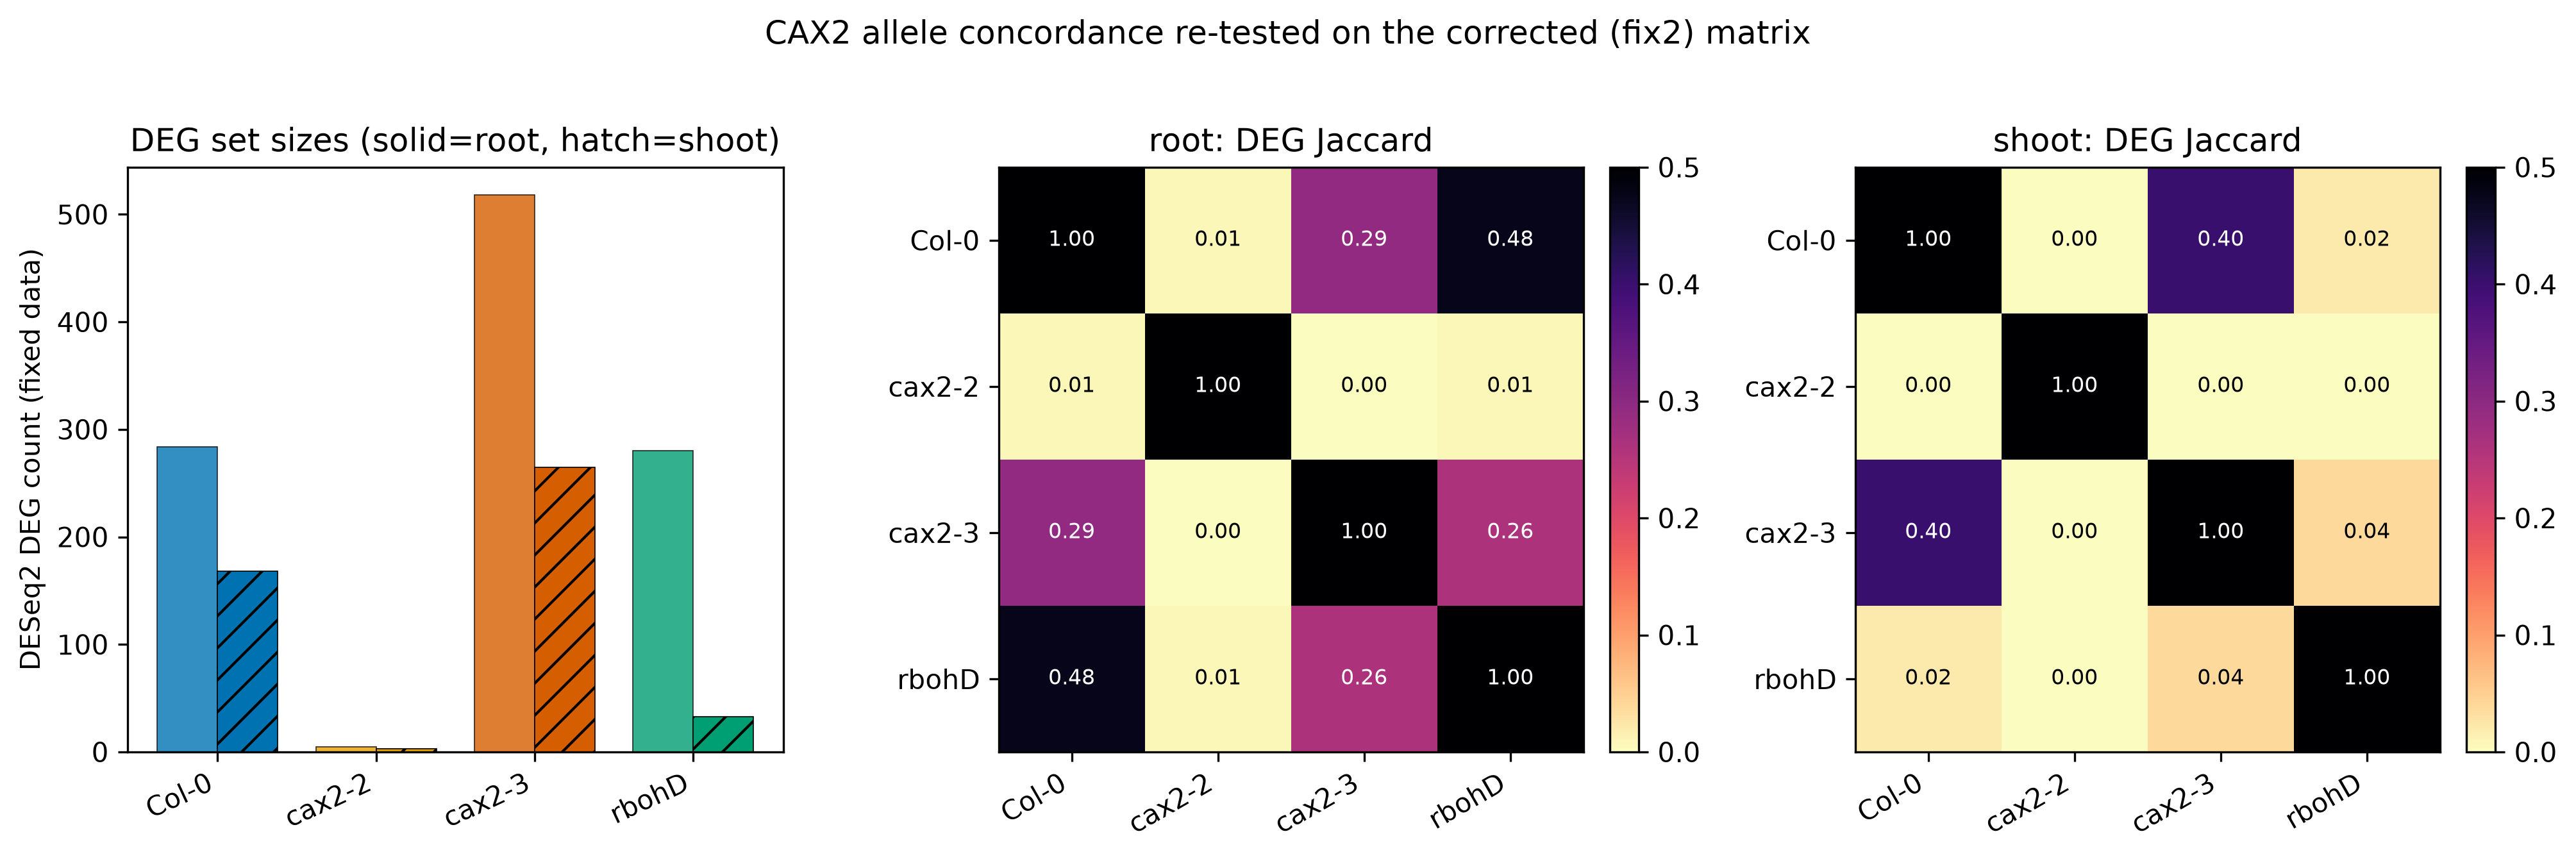
\includegraphics[width=0.7\textwidth]{figF1_cax2_concordance_fixed.png}
\caption{\textbf{\textit{cax2-3} exclusion (corrected data).} The excluded fourth
genotype's flight-DEG set inflated \(\sim 90\)--100\(\times\) relative to
\textit{cax2-2} with an outlier library --- a technical artefact.}
\label{fig:s1}
\end{figure}

\begin{figure}[htbp]
\centering
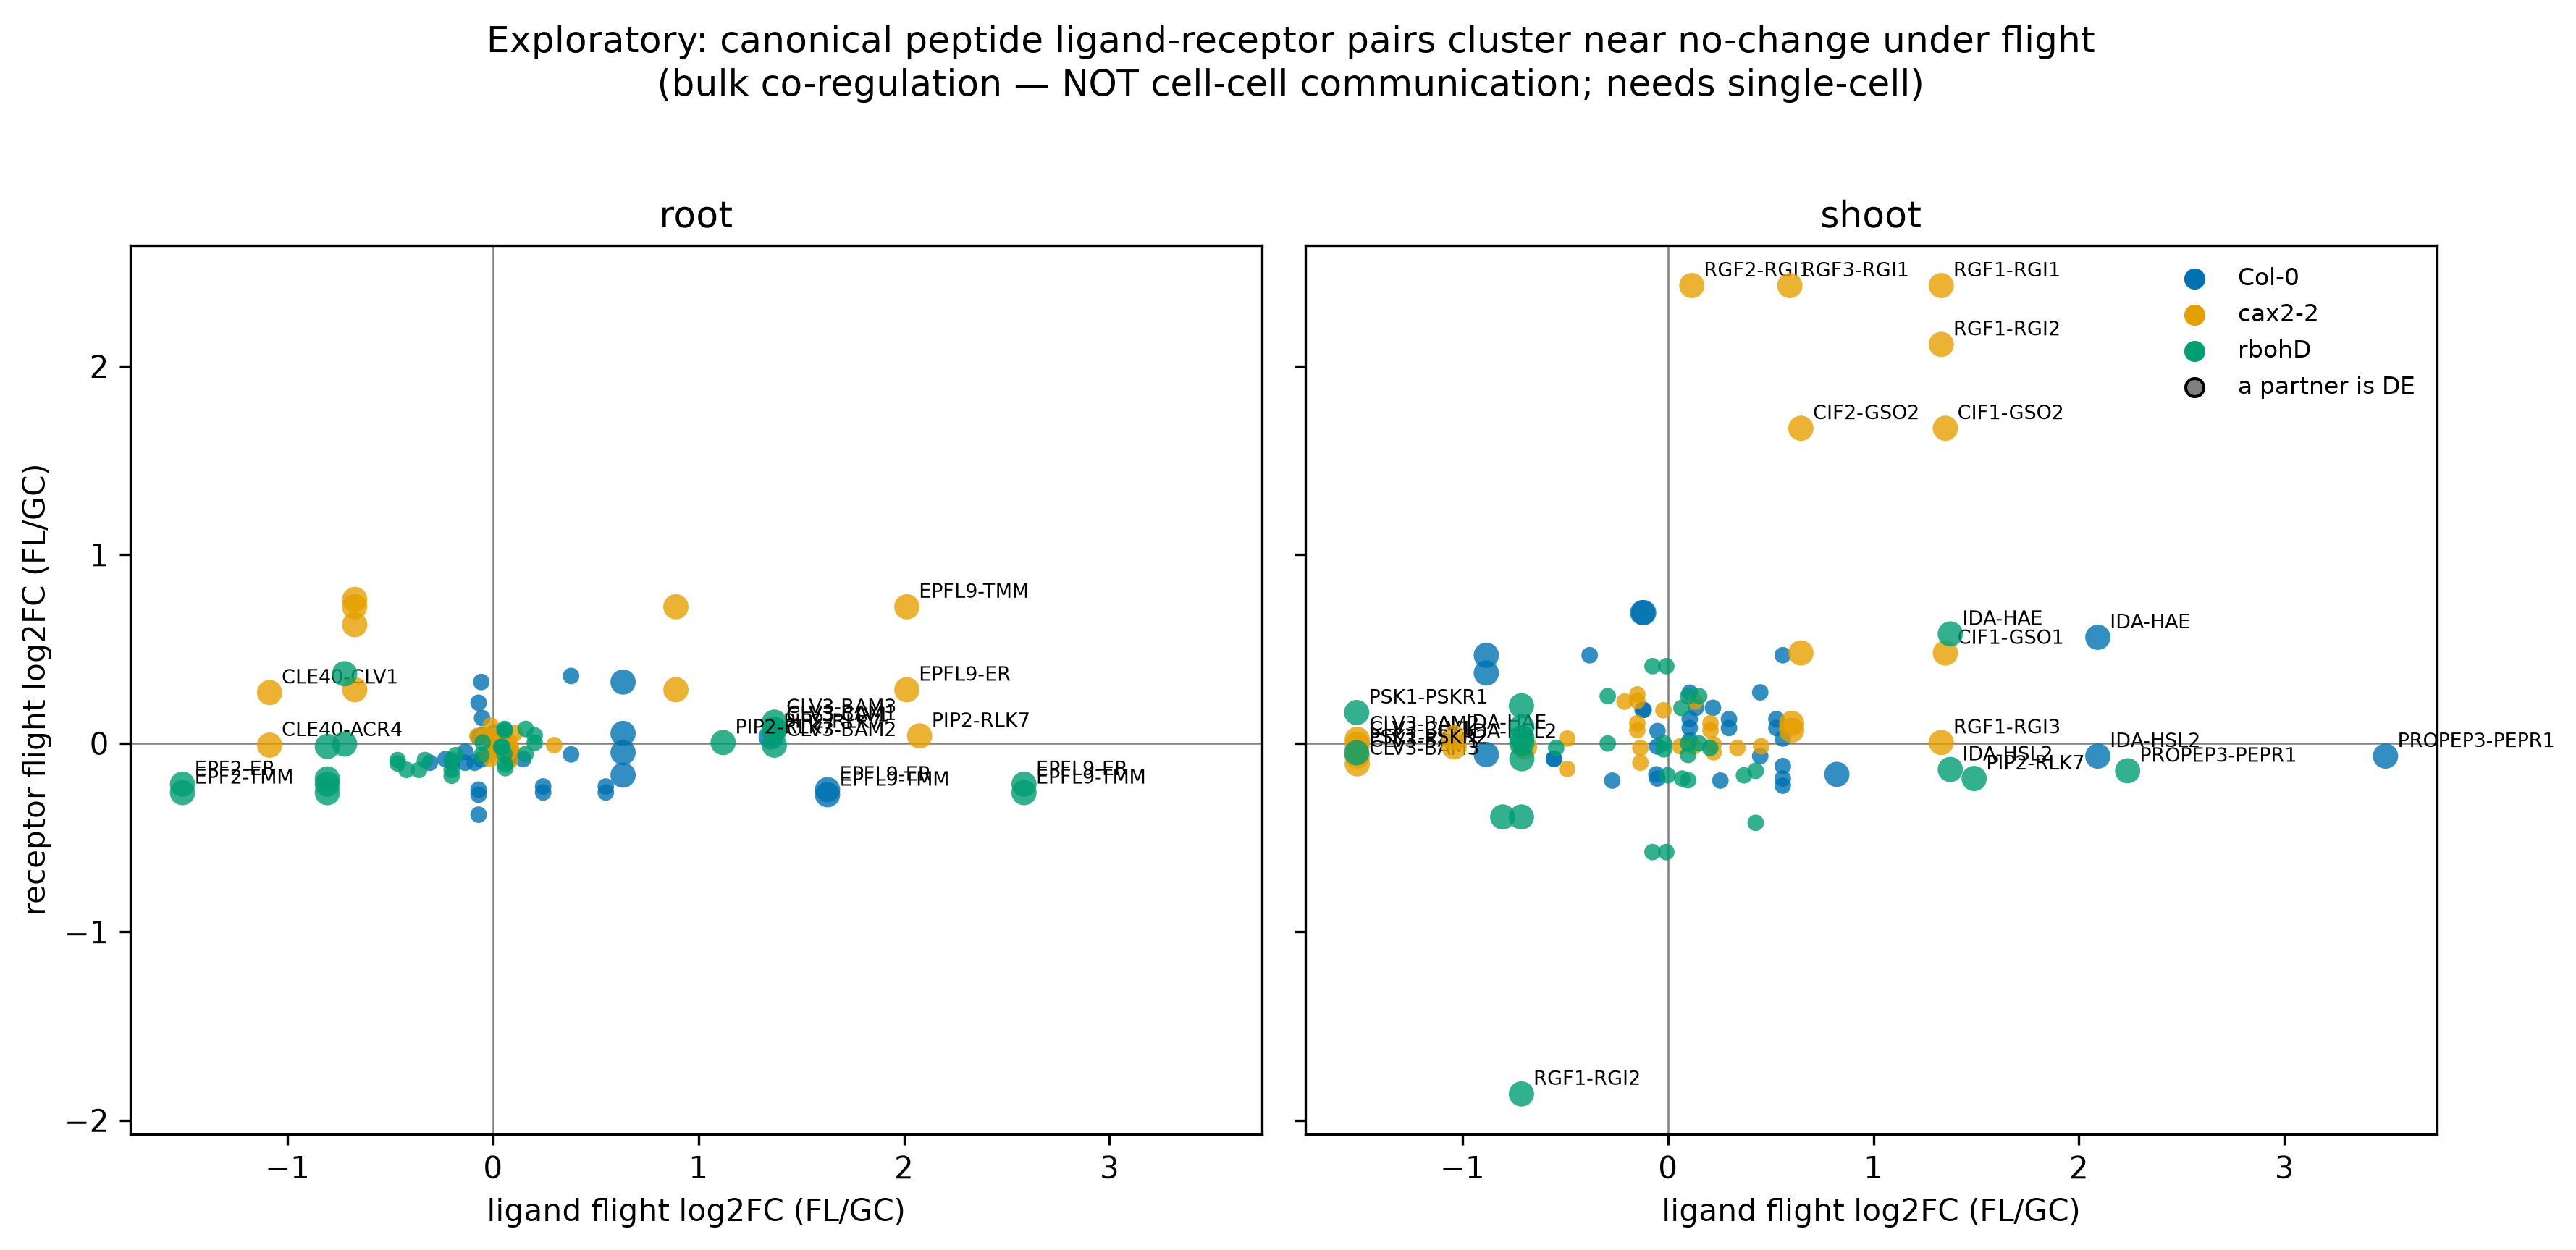
\includegraphics[width=0.7\textwidth]{figN1_ligand_receptor.png}
\caption{\textbf{Exploratory peptide ligand--receptor flight-responsiveness.} No
module had both partners pass the DE threshold; peptide-signalling genes cluster near
no-change.}
\label{fig:s2}
\end{figure}

\begin{figure}[htbp]
\centering
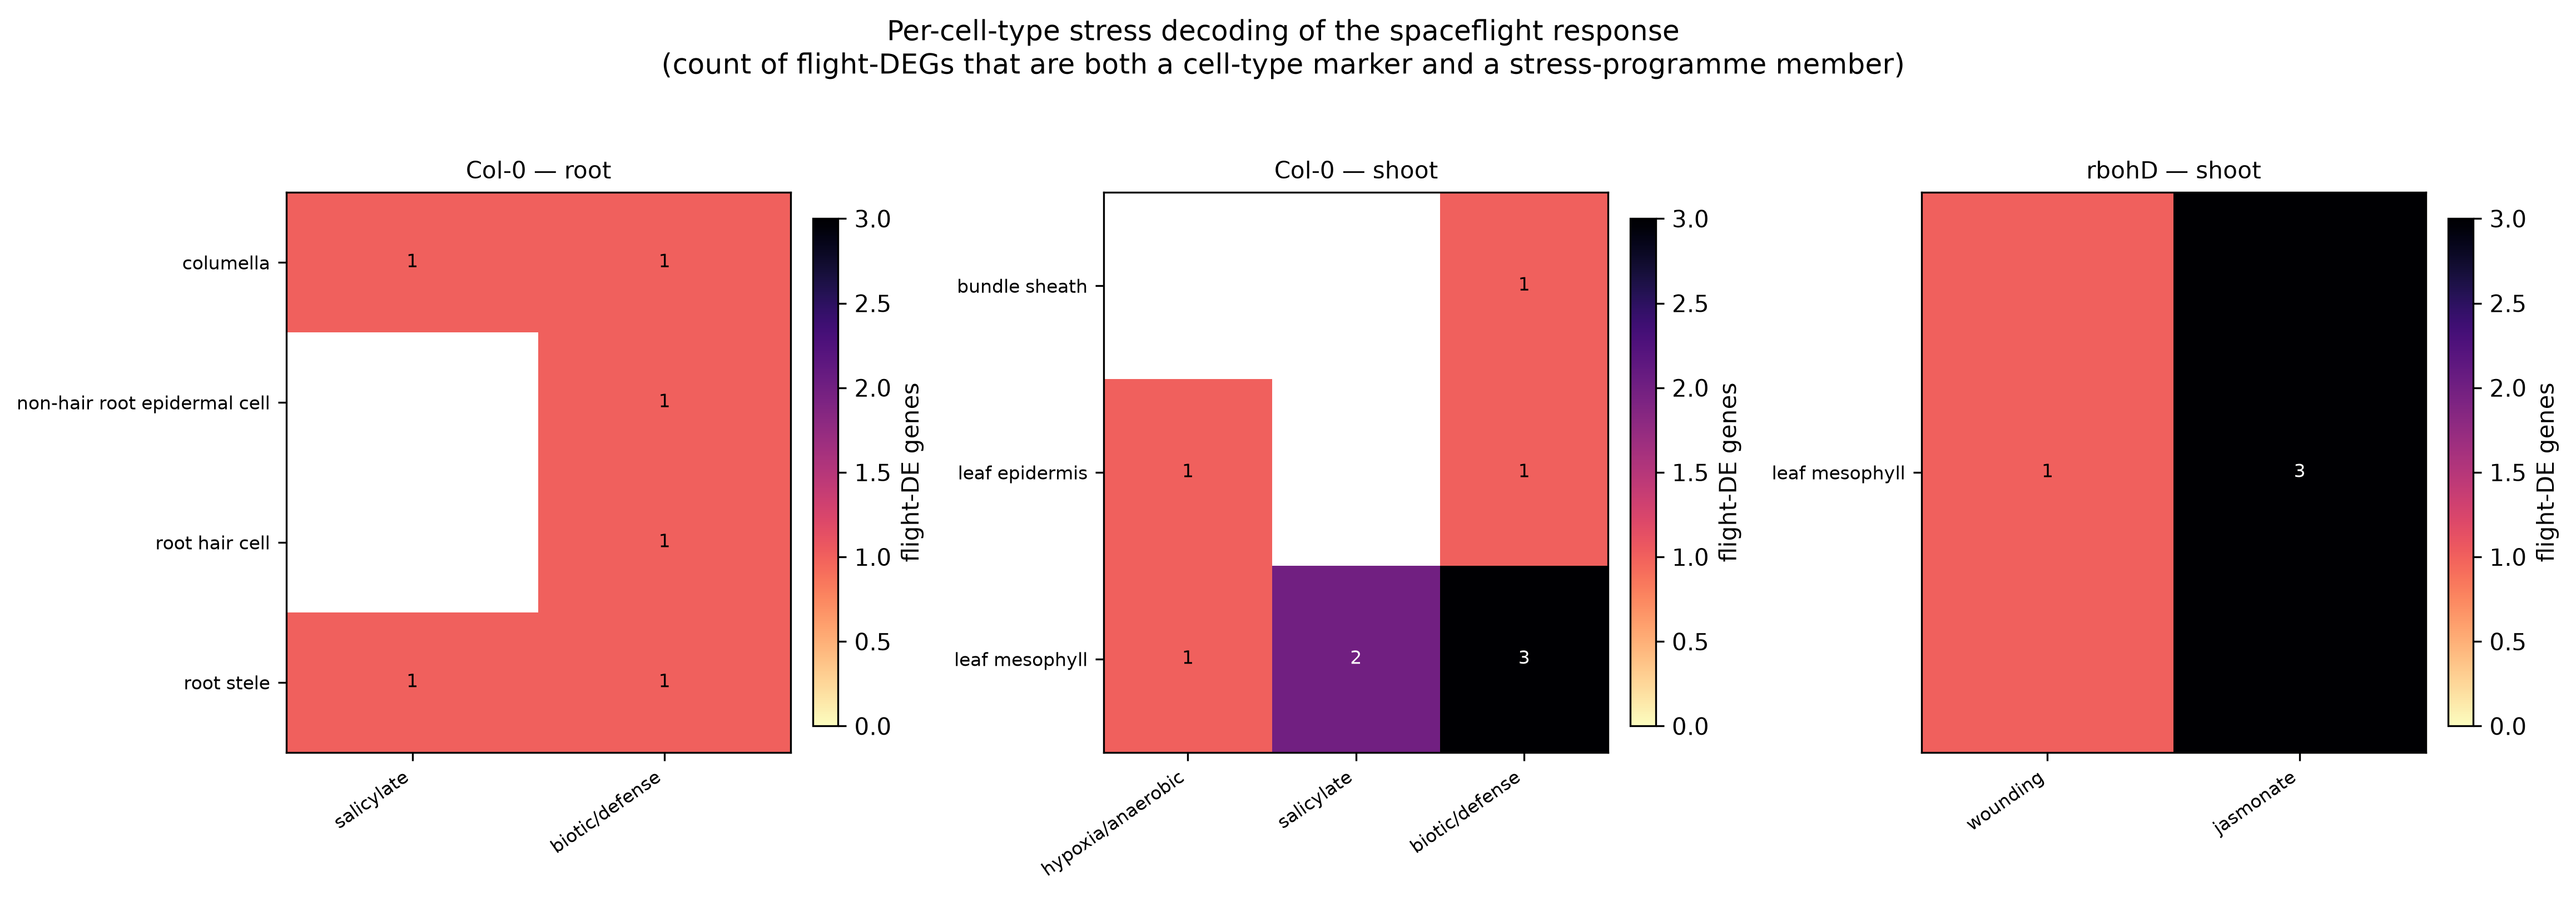
\includegraphics[width=0.85\textwidth]{figL2_celltype_stress_decoding.png}
\caption{\textbf{Cell-type-resolved stress decoding.} For each significant stress
programme (Fig.~\ref{fig:7}), member flight-DEGs are attributed to cell types via the
PCMDB markers. The defence/hormone signature localises chiefly to leaf mesophyll.}
\label{fig:s3}
\end{figure}

\begin{figure}[htbp]
\centering
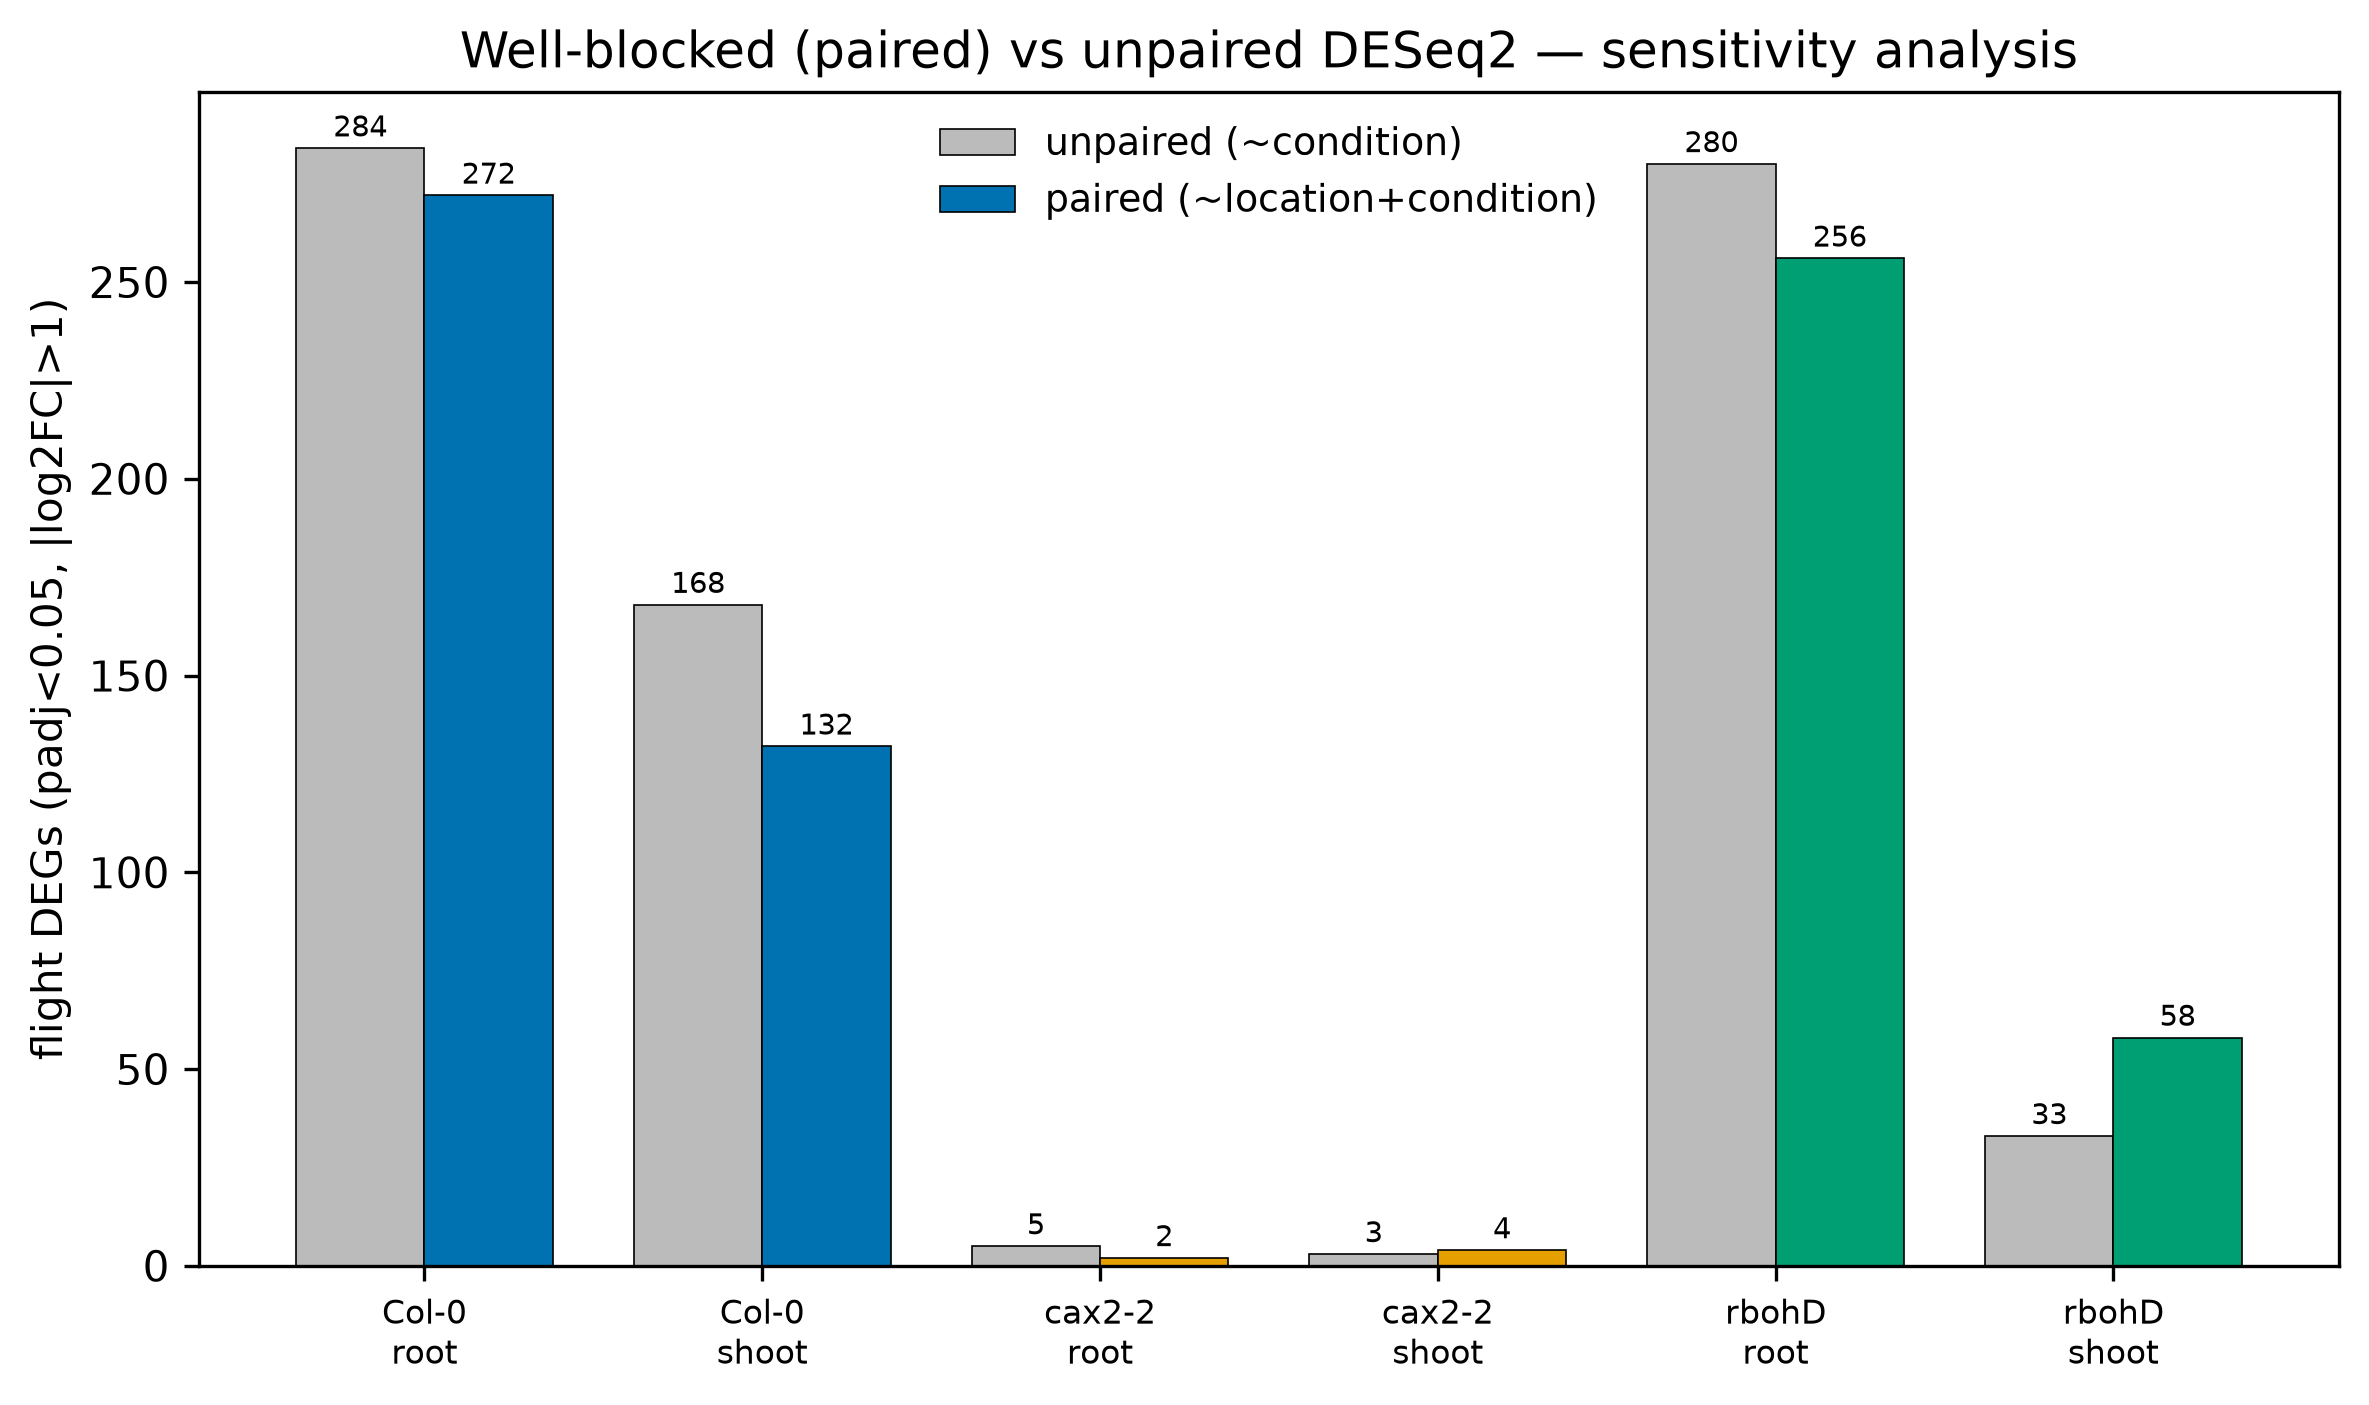
\includegraphics[width=0.7\textwidth]{figO1_paired_vs_unpaired_DEGs.png}
\caption{\textbf{Well-blocked (paired) DESeq2 --- sensitivity analysis.} Flight-DEG
counts from the unpaired model (\(\sim\)condition) vs a paired model blocking on
plate well (\(\sim\)location + condition). Counts are broadly concordant and every
qualitative conclusion is unchanged.}
\label{fig:s4}
\end{figure}

\begin{figure}[htbp]
\centering
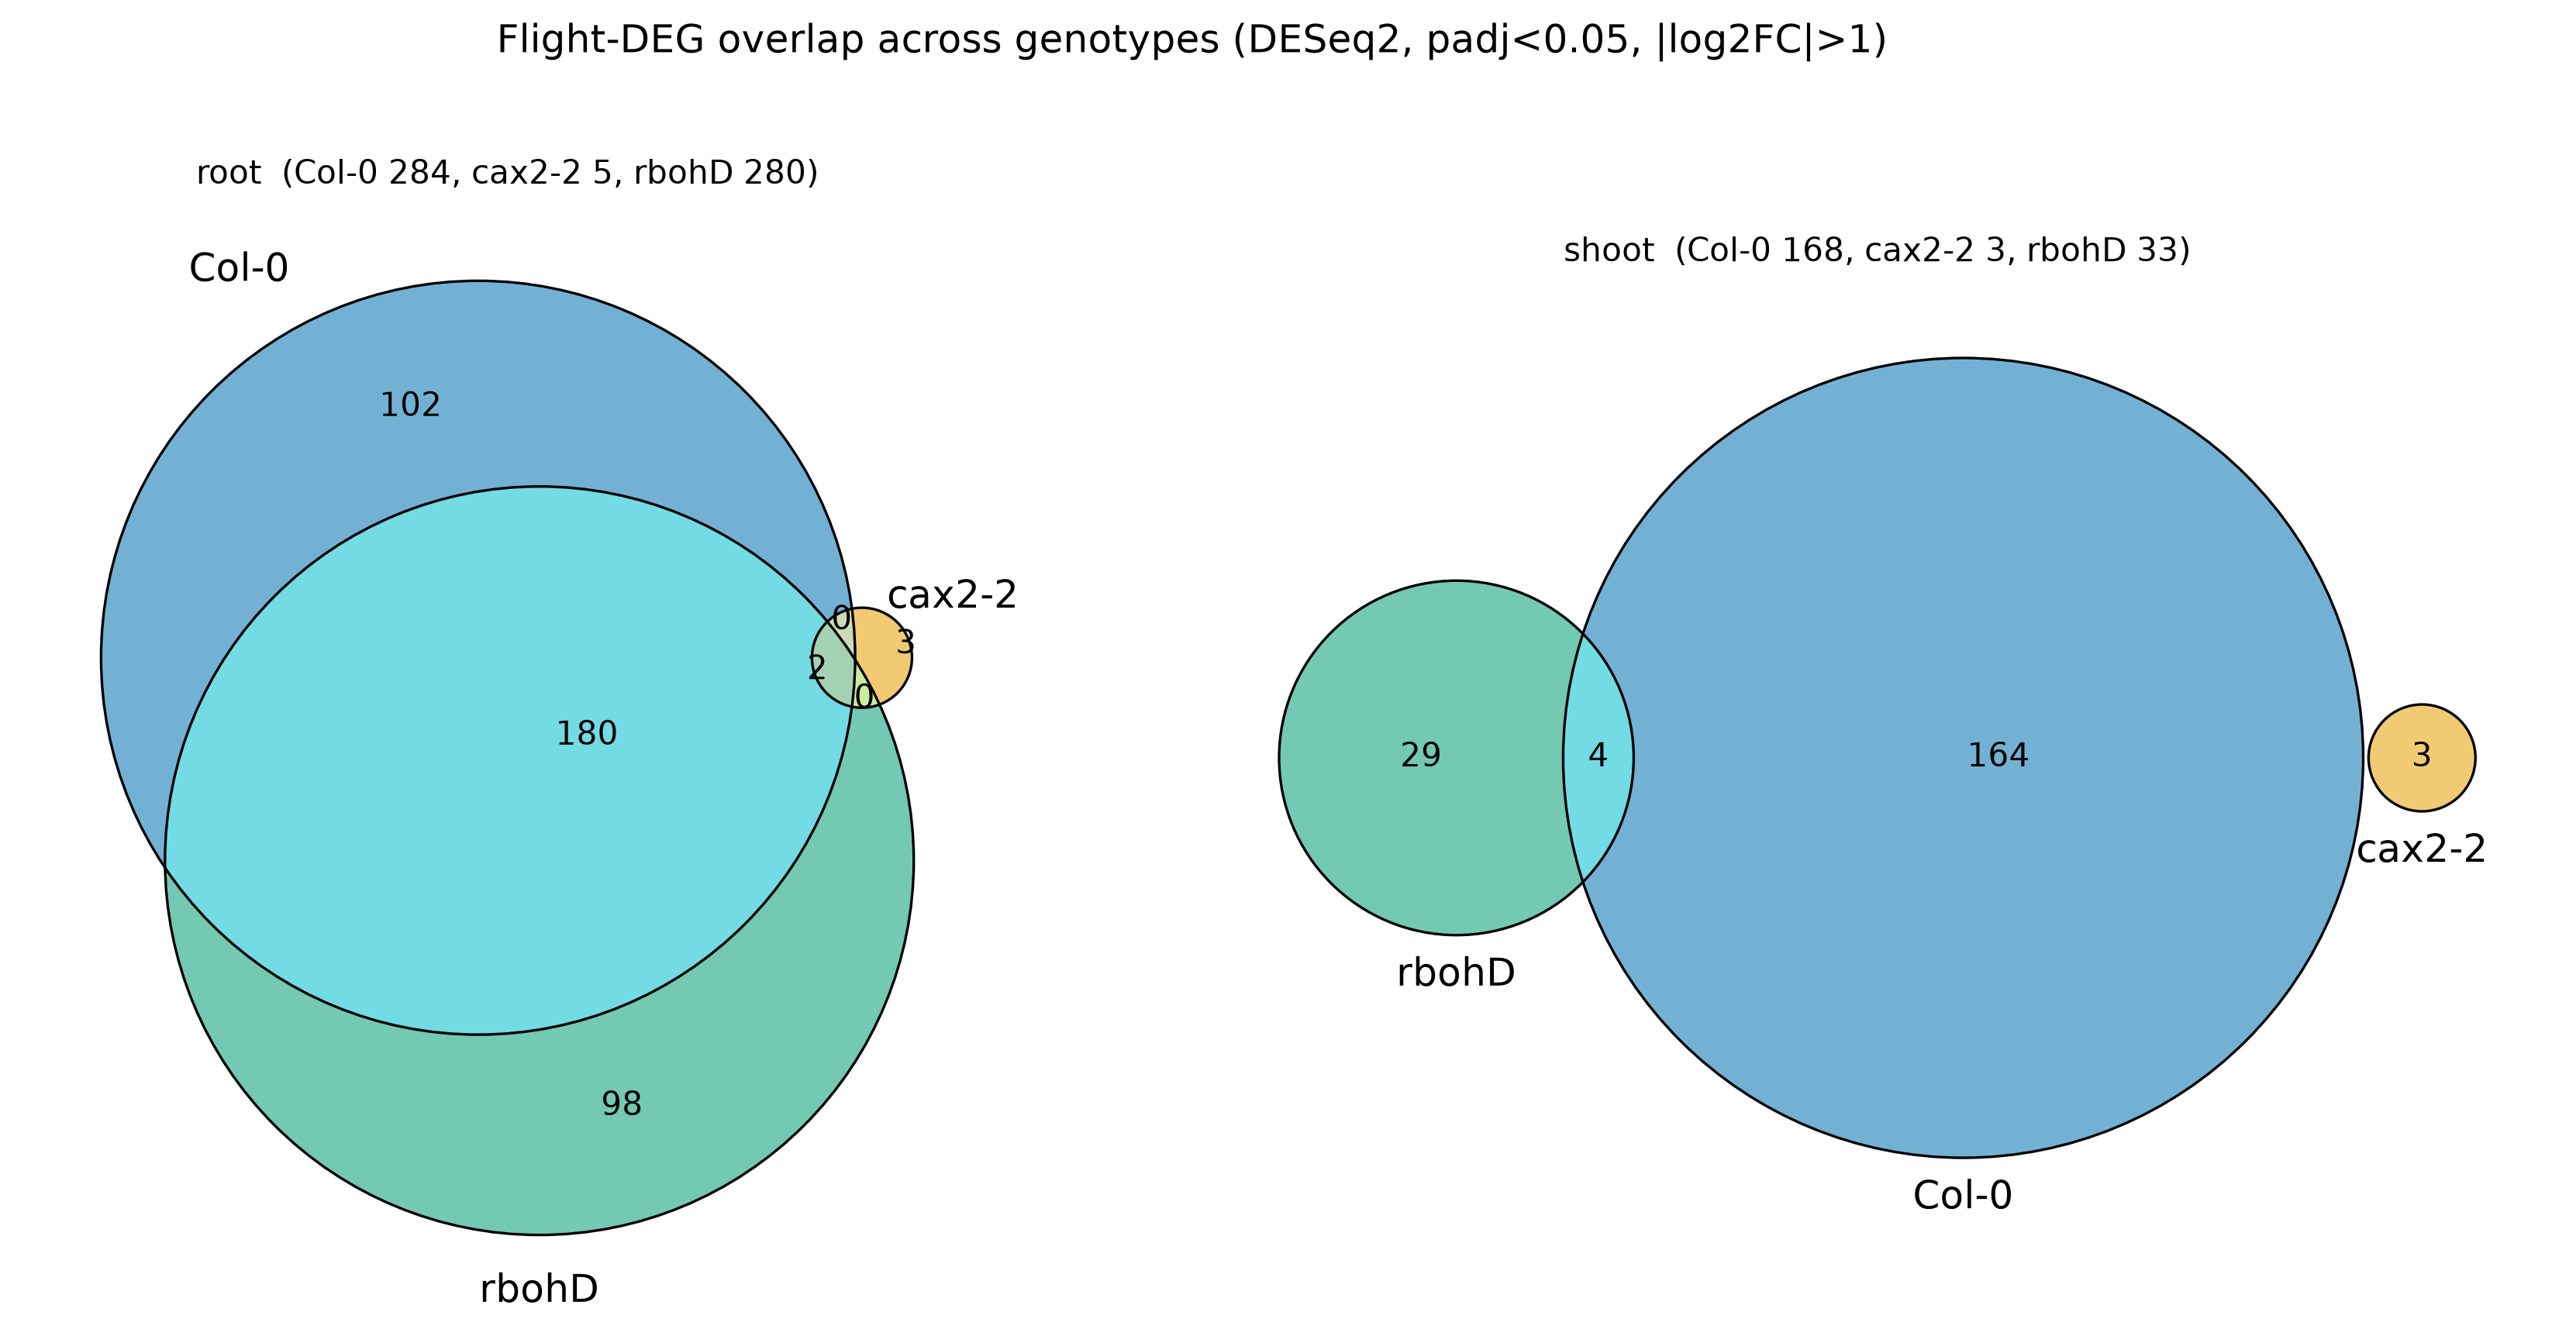
\includegraphics[width=0.7\textwidth]{figP1_deg_overlap_venn.png}
\caption{\textbf{Flight-DEG overlap across genotypes.} Three-way Venn of the DESeq2
flight-DEG sets (Col-0, \textit{cax2-2}, \textit{rbohD}) for root and shoot. Wild type
and \textit{rbohD} share a 180-gene root flight core; only 2 genes are shared by all
three; \textit{cax2-2} is near-empty.}
\label{fig:s5}
\end{figure}

\end{document}
